\documentclass[onecolumn]{IEEEtran}

\usepackage[utf8]{inputenc}
\usepackage[T1]{fontenc}
\usepackage{mathtools}
\usepackage{amssymb}
\usepackage{amsmath}

\numberwithin{equation}{section}
\DeclareMathOperator*{\argmax}{arg\,max}
\DeclareMathOperator*{\argmin}{arg\,min}
\DeclareMathOperator{\diag}{diag}

\usepackage{amsthm}
\usepackage{thmtools}

\newtheorem{theorem}{Theorem}[section]
\newtheorem{lemma}[theorem]{Lemma}
\newtheorem{corollary}[theorem]{Corollary}
\newtheorem{proposition}[theorem]{Proposition}

\theoremstyle{definition}
\newtheorem{definition}[theorem]{Definition}
\newtheorem{example}[theorem]{Example}

\theoremstyle{remark}
\newtheorem{remark}[theorem]{Remark}
\newtheorem*{note}{Note}

\usepackage{booktabs}
\usepackage{array}
\usepackage{multirow}
\usepackage{tabularx}
\usepackage{longtable}
\usepackage{siunitx}

\newcolumntype{C}[1]{>{\centering\arraybackslash}p{#1}}
\newcolumntype{L}[1]{>{\raggedright\arraybackslash}p{#1}}
\sisetup{
    table-format = 3.2,
    table-auto-round = true
}

\usepackage{tikz}
\usepackage{pgfplots}
\pgfplotsset{compat=1.18}

\usetikzlibrary{
  arrows.meta,
  positioning,
  shapes.geometric,
  shadows,
  fit,
  calc,
  matrix,
  shapes.misc
}
\tikzset{
  base/.style = {rectangle, rounded corners, draw=black, minimum width=2.5cm, minimum height=1cm, text centered, font=\sffamily},
  startstop/.style = {base, fill=red!20, drop shadow},
  process/.style = {base, fill=blue!20, drop shadow},
  decision/.style = {diamond, aspect=1.5, draw=black, fill=green!20, drop shadow, align=center},
  arrow/.style = {thick, -{Stealth[length=3mm]}},
  matrix_style/.style={matrix of nodes, row sep=0.5cm, column sep=0.5cm, nodes={anchor=center}},
  dashdot/.style={dash pattern=on 3pt off 3pt on 1pt off 3pt}
}

\usepackage{algorithm}
\usepackage{algorithmicx}
\usepackage{algpseudocode}

\algrenewcommand\algorithmicrequire{\textbf{Input:}}
\algrenewcommand\algorithmicensure{\textbf{Output:}}

\usepackage{graphicx}
\usepackage{url}
\usepackage{xcolor}
\usepackage{caption}
\usepackage[colorlinks=true, linkcolor=blue, citecolor=green!50!black, urlcolor=blue!80!black]{hyperref}

\IEEEoverridecommandlockouts

% Draft watermark removed for empirical camera-ready manuscript
\newsavebox{\tikzfitbox}
\newcommand{\fitwidth}[1]{%
  \sbox{\tikzfitbox}{#1}%
  \ifdim\wd\tikzfitbox>\linewidth
    \resizebox{\linewidth}{!}{\usebox{\tikzfitbox}}%
  \else
    \usebox{\tikzfitbox}%
  \fi
}
\begin{document}

\title{CMA-SAM: Cross-Modal Anchor Generation for Text-Driven Medical Image Segmentation}

\maketitle

\begin{abstract}
Medical image segmentation is a critical component of clinical diagnosis and surgical planning, yet it is often bottlenecked by the scarcity of high-quality annotations and the exorbitant costs of manual labeling. While Vision Foundation Models, particularly the Segment Anything Model (SAM), have demonstrated remarkable zero-shot capabilities, their application in medical imaging traditionally relies on explicit, manually crafted geometric prompts (e.g., points or bounding boxes). Recent vision-language adaptations attempt to replace manual prompts with text queries; however, they typically bypass SAM's highly optimized geometric prompt encoder by forcing the mask decoder to resolve spatial boundaries directly from continuous, dense cross-modal embeddings. This often leads to suboptimal boundary delineation and spatial hallucinations in complex anatomical structures. To address this limitation, we propose the Cross-Modal Anchor Segment Anything Model (CMA-SAM), a novel framework that seamlessly bridges continuous semantic text embeddings with discrete geometric prompts. CMA-SAM leverages implicit cross-modal specification and joint feature fusion to autonomously regress optimal geometric anchors. Specifically, visual features and simple text queries are fused via bidirectional cross-attention, and a novel Autonomous Anchor Generation (AAG) module employs a differentiable spatial softmax operation to predict precise point coordinates and bounding boxes. By feeding these autonomously generated discrete anchors directly into SAM's native prompt encoder, CMA-SAM explicitly decouples semantic localization from high-frequency boundary delineation. This approach eliminates the need for manual prompt engineering while fully exploiting SAM's pre-trained coordinate-based decoding strengths. Extensive experiments on endoscopic (Kvasir-SEG) and dermoscopic (ISIC 2018) benchmarks demonstrate that CMA-SAM reduces Anchor Localization Error by 88.2\%--94.0\% over visual saliency self-prompting (down to 3.92 and 1.30 grid pixels), improves cross-domain few-shot segmentation by up to 34.56 percentage points in 1-shot adaptation, compresses over $10^6$ continuous dense feature activations into at most 24 interpretable spatial coordinates while retaining over 99.3\% of dense-decoding in-domain accuracy, and exhibits $11.4\times$ higher stability across simple versus complex clinical text prompts at 4.54M trainable parameters.
\end{abstract}

\begin{IEEEkeywords}
Medical Image Segmentation, Segment Anything Model (SAM), Vision-Language Models, Autonomous Anchor Generation, Cross-Modal Alignment, Zero-Shot Segmentation, Prompt Engineering
\end{IEEEkeywords}

\section{Introduction}

\subsection{Background: Foundation Models in Medical Image Segmentation}

Medical image segmentation is a cornerstone of modern clinical workflows, serving as a critical prerequisite for automated diagnostics, disease staging, and surgical planning. By precisely delineating anatomical structures and pathological lesions at the pixel level, automated segmentation systems significantly reduce the cognitive load on clinicians and minimize inter-observer variability \cite{defauw2018clinically}. As healthcare systems increasingly adopt data-driven diagnostic pipelines, the demand for robust, scalable, and highly accurate segmentation models has grown exponentially. However, the deployment of these systems across multi-institutional settings is often hindered by the vast heterogeneity of medical imaging modalities, varying clinical protocols, and the inherent challenges associated with decentralized data distributions \cite{sheller2019multi}.

To address the limitations of traditional, task-specific models trained on narrow datasets, the field has recently witnessed a paradigm shift driven by the advent of Vision Foundation Models (VFMs). Foremost among these is the Segment Anything Model (SAM) \cite{kirillov2023segment}, which has redefined the landscape of image segmentation through its unprecedented zero-shot generalization capabilities. Pre-trained on a massive corpus of natural images, SAM utilizes explicit geometric prompts—such as point clicks and bounding boxes—to interactively extract highly precise object masks. The introduction of SAM has catalyzed extensive research into its applicability within the medical domain \cite{ma2024segment}. However, comprehensive empirical evaluations have consistently revealed that while SAM exhibits remarkable potential, its out-of-the-box performance frequently degrades when confronted with the low contrast, ambiguous boundaries, and complex tissue architectures inherent to medical images \cite{mazurowski2023segment, huang2024segment}.

Concurrently, the rapid evolution of Vision-Language Models (VLMs) has opened new avenues for cross-modal semantic reasoning. Models such as the Contrastive Language-Image Pre-training (CLIP) framework \cite{radford2021learning} and its domain-specific adaptations like BiomedCLIP \cite{zhang2025biomedclip} have demonstrated profound capabilities in aligning high-dimensional visual features with rich textual semantics. By mapping images and natural language descriptions into a shared, continuous latent space, VLMs offer a powerful mechanism for zero-shot classification and semantic grounding. The integration of these cross-modal capabilities into medical imaging holds immense potential for developing universal foundation models \cite{lee2024foundation}. Such models promise to transcend the limitations of purely visual heuristics by leveraging the vast clinical knowledge embedded in text, thereby enabling more interpretable, context-aware, and automated diagnostic systems \cite{bommasani2022opportunities}.

\subsection{Problem Definition: The Semantic-to-Spatial Gap and Prompting Limitations}
\label{sec:promising_gaps}

Despite the remarkable zero-shot capabilities of vision foundation models, their direct application to the medical domain is severely bottlenecked by a reliance on explicit, manual geometric prompts, such as point clicks or bounding boxes. Monolithic adaptations of the Segment Anything Model (SAM), which fine-tune the visual encoder for medical images, still fundamentally depend on these manual inputs to localize targets \cite{zhang2023customized, cheng2024unleashing, wu2025medical}. Acquiring these explicit geometric specifications is prohibitively expensive, requiring continuous human-in-the-loop intervention from clinical experts. Furthermore, in highly heterogeneous medical tissues—such as diffuse tumors or noisy ultrasound scans—a single geometric point is often ambiguous. This ambiguity frequently causes the model to capture irrelevant adjacent structures or fail to delineate the full extent of the lesion, necessitating complex prompt augmentation strategies that still fall short of true autonomy \cite{dai2024samaug}.

To circumvent the exorbitant costs of manual geometric prompting, recent research has pivoted toward text-driven segmentation. However, existing methodologies in this space typically demand highly complex, expert-crafted clinical descriptions to function effectively. Models relying on explicit textual specification or sequential cascading architectures require semantically rich diagnostic text to disambiguate anatomical structures \cite{koleilat2025medclip, wang2022medclip, li2024clipsam}. For instance, reducing the input to a simple class name (e.g., ``polyp'' or ``melanoma'') often results in severe performance degradation. The necessity for exhaustive linguistic input limits the scalability and real-world deployment of these models, as generating detailed clinical text for every diagnostic frame is just as impractical as manual point clicking in fast-paced clinical environments.

Recognizing the limitations of both manual geometric coordinates and complex clinical text, the most recent wave of foundation model adaptations has explored implicit cross-modal specification. These methods leverage joint feature fusion to synthesize guidance signals from simple text queries \cite{qian2024simplevilmedsam, aleem2024test, wang2024sam, lan2024proxyclip}. While this approach successfully eliminates the need for complex prompt engineering, it introduces a critical algorithmic flaw: the reliance on direct dense decoder projection or continuous attribution maps \cite{wang2023visual}. By forcing the network to decode high-frequency spatial boundaries directly from abstract, continuous cross-modal embeddings, these architectures bypass SAM's highly optimized discrete geometric prompt encoder. This continuous-to-continuous translation forces the mask decoder to simultaneously solve global semantic localization and local boundary delineation. Consequently, these methods frequently suffer from spatial hallucinations and suboptimal boundary delineation, particularly when confronted with structurally complex medical lesions. They fail to bridge the fundamental semantic-to-spatial gap because they do not provide the mask decoder with the exact modality of input—discrete spatial coordinates—that it was explicitly pre-trained to process most efficiently.

\subsection{Our Contribution: Cross-Modal Anchor Segment Anything Model (CMA-SAM)}

To address the aforementioned limitations, we propose the Cross-Modal Anchor Segment Anything Model (CMA-SAM). This novel framework is explicitly designed to bridge the semantic-to-spatial gap in medical image segmentation using only simple text queries, such as basic anatomical or disease-related class names. By deeply coupling the visual encoding capabilities of foundation models with cross-modal semantic understanding, CMA-SAM eliminates the dependency on both manual geometric prompts and complex, expert-crafted clinical text descriptions.

The core innovation of our framework is the Autonomous Anchor Generation (AAG) module. Instead of forcing the mask decoder to resolve high-frequency spatial boundaries directly from abstract, continuous cross-modal embeddings, the AAG module translates these continuous features into discrete geometric anchors—specifically, a set of optimal point prompts and a global bounding box. This translation is achieved through a fully differentiable Spatial Softmax operation, which allows the network to mathematically regress exact spatial coordinates while remaining end-to-end optimizable via backpropagation.

This mathematically rigorous, cross-modal anchor regression mechanism stands in stark contrast to existing autonomous prompting methods. Current self-prompting architectures typically rely on non-differentiable visual heuristics, such as image saliency thresholding or edge detection, operating entirely within a monolithic, vision-only paradigm \cite{xie2025self, chen2024un, shaharabany2023autosam, wu2023self}. Because these heuristic methods lack explicit semantic guidance, they frequently fail in heterogeneous medical images where the clinical target is not the most visually salient object in the frame. CMA-SAM overcomes this critical flaw by ensuring that the generated discrete prompts are deeply grounded in the semantic intent provided by the text query.

In summary, the key contributions of our work are threefold:
\begin{itemize}
    \item We introduce a novel semantic-to-spatial translation paradigm that eliminates the bottleneck of manual prompt engineering while fully preserving the highly optimized, discrete geometric decoding efficiency native to SAM \cite{kirillov2023segment}.
    \item We propose the AAG module, which effectively mitigates the spatial hallucinations and boundary blurring inherent in direct dense decoding architectures by forcing the model to commit to explicit, interpretable spatial coordinates before final mask generation.
    \item We establish theoretical gradient-flow, localization-error, and information-bottleneck bounds for expectation-based anchor generation, and empirically validate CMA-SAM on gastrointestinal endoscopy (Kvasir-SEG \cite{jha2020kvasir}) and dermoscopy (ISIC 2018 \cite{codella2018skin}), demonstrating substantial gains in cross-domain few-shot efficiency, anchor localization precision, and robustness to text prompt complexity.
\end{itemize}

\subsection{Paper Organization}

The remainder of this paper is organized as follows. Section II reviews related work across monolithic foundation model adaptation, explicit and implicit cross-modal specification, and autonomous prompt engineering \cite{ali2023prompt, shang2024prompt, ji2024segment}. Section III details the proposed CMA-SAM architecture, including LoRA-adapted visual encoding, bidirectional cross-attention fusion, bounded Spatial Softmax anchor regression, and mask-derived geometric anchor supervision. Section IV establishes formal theoretical bounds on Spatial Softmax differentiability, modality-gap localization error, information-theoretic background filtering, and asymptotic complexity. Section V presents comprehensive quantitative and qualitative experiments, ablations, and efficiency benchmarks \cite{milletari2016vnet, ma2021loss}. Finally, Section VI concludes the paper and outlines future research directions.
\section{Related Work}

\subsection{Explicit Geometric Specification and Monolithic Adaptation}

The advent of Vision Foundation Models (VFMs) has fundamentally reshaped the landscape of image segmentation. The Segment Anything Model (SAM) \cite{kirillov2023segment} established a new paradigm by demonstrating remarkable zero-shot generalization capabilities driven by explicit geometric specification, such as point clicks and bounding boxes. However, the direct application of SAM to the medical domain immediately exposed significant limitations. Comprehensive empirical evaluations by Mazurowski et al. \cite{mazurowski2023segment}, Huang et al. \cite{huang2024segment}, Ji et al. \cite{ji2024segment}, and Ma et al. \cite{ma2024segment} consistently demonstrated that out-of-the-box SAM struggles with the low contrast, ambiguous boundaries, and complex anatomical structures inherent to medical imaging modalities. Chen et al. \cite{chen2023sam} further corroborated these findings, highlighting that SAM's reliance on direct decoder projection fails to resolve fine-grained medical targets without domain-specific recalibration.

To overcome these zero-shot deficiencies, the research community heavily pivoted toward monolithic adaptation strategies. These approaches maintain SAM as a standalone, single-modality foundation model but introduce parameter-efficient fine-tuning (PEFT) mechanisms to inject medical domain knowledge. A pioneering work in this space is SAMed \cite{zhang2023customized}, which applied Low-Rank Adaptation (LoRA) to the SAM image encoder, enabling competitive performance on medical datasets while updating only a fraction of the model's parameters. Building on this, the Medical SAM Adapter \cite{wu2025medical} and AdaptiveSAM \cite{paranjape2023adaptivesam} integrated specialized adapter modules within the transformer blocks to better capture high-frequency local features crucial for medical image analysis. Furthermore, Hu et al. \cite{hu2023how} provided a systematic investigation into optimal fine-tuning pathways for SAM, while Cheng et al. \cite{cheng2023sam} developed comprehensive medical-specific adaptations. While these monolithic adaptations significantly improve visual feature extraction, they remain fundamentally tethered to the requirement of explicit geometric prompts provided by human experts.

Recognizing the bottleneck of manual prompt engineering, subsequent research attempted to augment the interaction between the geometric prompts and the monolithic architecture. H-SAM \cite{cheng2024unleashing} introduced a hierarchical decoding mechanism to better utilize multi-scale features, mitigating some of the spatial ambiguities caused by sparse point prompts. Similarly, SAMAug \cite{dai2024samaug} proposed visual and prompt augmentation techniques to enhance the robustness of the mask decoder against suboptimal point placements. Other works, such as those by Ali et al. \cite{ali2023prompt} and Shang et al. \cite{shang2024prompt}, explored algorithmic prompt engineering to optimize the spatial coordinates fed into SAM. Despite these enhancements, the core semantic-to-spatial translation mechanism remains a direct decoder projection, which lacks an interpretable intermediate spatial prior and still demands explicit spatial initialization.

The most advanced monolithic approaches have attempted to bypass human intervention entirely through heuristic-driven prompt generation. AutoSAM \cite{shaharabany2023autosam} and various self-prompting frameworks \cite{wu2023self} utilize auxiliary convolutional networks or image saliency heuristics to autonomously generate proxy geometric prompts. However, because these methods operate within a monolithic, vision-only architecture, they suffer from a profound semantic deficit. They rely purely on visual contrast or pre-defined structural priors, making them highly susceptible to failure in heterogeneous tissues where the target is defined by complex clinical semantics (e.g., distinguishing a benign cyst from a malignant tumor) rather than mere visual saliency. 

\textbf{Critical Analysis and Alignment with Research Gaps:} 
The trajectory of the aforementioned literature perfectly illustrates the limitations of combining \textit{Explicit Geometric Specification} with \textit{Monolithic Adaptation}. While parameter-efficient fine-tuning \cite{zhang2023customized, wu2025medical} solves the domain shift problem at the visual feature level, it does not solve the semantic grounding problem. The reliance on explicit geometric prompts restricts scalability, and attempts to automate these prompts \cite{shaharabany2023autosam, wu2023self} fail because they lack cross-modal semantic guidance. 

This critical shortcoming directly motivates the research gaps identified in our Dynamic MECE framework. To achieve truly automated, semantically aware medical segmentation, the field must transition away from monolithic vision-only models. Instead, as proposed in our CMA-SAM methodology, we must leverage \textit{Implicit Cross-Modal Specification} (using Vision-Language Models to provide semantic understanding) coupled with \textit{Autonomous Anchor Generation}. By doing so, we can synthesize the zero-shot semantic localization capabilities of text-driven models with the highly optimized, discrete geometric decoding efficiency of SAM \cite{kirillov2023segment}, effectively bridging the semantic-to-spatial divide without requiring manual prompt engineering.

\subsection{Explicit Textual Specification via Joint Feature Fusion and Sequential Cascading}

The integration of natural language processing \cite{chowdhary2020natural} into medical imaging has catalyzed a paradigm shift from manual geometric prompting to text-driven segmentation. To disambiguate complex anatomical structures and heterogeneous lesions, many current state-of-the-art methods rely on \textit{Explicit Textual Specification}. This approach requires semantically rich, expert-crafted clinical descriptions to guide the vision foundation model. Recently, the generation of these detailed prompts has been increasingly augmented by specialized medical large language models \cite{sellergren2025medgemma}, which synthesize comprehensive diagnostic text. However, the architectural strategies employed to integrate these explicit textual prompts with visual features broadly bifurcate into two distinct categories within our MECE framework: Sequential Cascading and Joint Feature Fusion.

Sequential Cascading architectures decouple the vision and language processing stages into a multi-step pipeline. For instance, ClipSAM \cite{li2024clipsam} employs a cascaded approach where a vision model first generates class-agnostic region proposals, which are subsequently filtered, classified, or refined by a vision-language model based on the explicit text prompt. While this modularity simplifies the training of individual components, it introduces significant computational redundancy. More critically, sequential pipelines suffer from irreversible error propagation; if the initial visual proposal stage fails to capture a subtle or diffuse lesion, the subsequent textual grounding stage cannot recover the lost spatial information, rendering the explicit text prompt entirely ineffective.

To overcome the inherent limitations of cascading, the field has largely pivoted toward \textit{Joint Feature Fusion}. Foundational works like MedCLIP \cite{wang2022medclip} and its broader biomedical adaptations \cite{liu2023clip, zhang2025biomedclip} demonstrated the profound efficacy of aligning medical images and clinical text within a shared, continuous latent space. Building upon these contrastive learning principles, unified medical vision-language frameworks \cite{fan2024medslip, khattak2024unimed} have been developed to enhance cross-modal representation learning prior to downstream segmentation tasks. 

In the specific context of adapting the Segment Anything Model (SAM), methods such as MedCLIP-SAM v2 \cite{koleilat2025medclip} and CLIP2SAM \cite{sun2024clip2sam} integrate these foundation models end-to-end. They utilize bidirectional cross-attention mechanisms to fuse explicit clinical text embeddings directly with SAM's dense visual features. Further algorithmic refinements in this domain include class-wise prompt generation strategies \cite{pu2025classwise}, multi-scale cross-modal bottleneck networks \cite{zhang2025mcbtnet} that attempt to preserve fine-grained semantics, and exploratory studies investigating the utility of diverse textual cues beyond standard diagnostic descriptions \cite{lin2024beyond, wang2024use}.

Despite the representational power of Joint Feature Fusion, a critical analysis reveals that these methodologies exhibit a fundamental algorithmic shortcoming: they predominantly rely on \textit{Direct Decoder Projection} for semantic-to-spatial translation. By forcing the mask decoder to directly resolve dense spatial boundaries from abstract, fused cross-modal embeddings, these models bypass the highly optimized discrete geometric prompt encoder native to SAM. This architectural choice leads to two major limitations:
\begin{itemize}
    \item \textbf{Sensitivity to Prompt Sparsity:} Because the spatial grounding relies entirely on the richness of the fused embedding, these models experience severe performance degradation when the explicit textual specification is reduced to simple class names. They fail to generalize to the \textit{Implicit Cross-Modal Specification} paradigm, demanding continuous expert linguistic input.
    \item \textbf{Suboptimal Boundary Delineation:} As identified in our research gap analysis (Section \ref{sec:promising_gaps}), the absence of an intermediate spatial prior or discrete anchor generation forces the mask decoder to simultaneously solve global semantic localization and local high-frequency boundary refinement. This dual burden often results in over-segmentation or blurred boundaries for structurally complex lesions.
\end{itemize}

Consequently, while explicit textual models \cite{koleilat2025medclip, li2024clipsam} achieve high accuracy when provided with exhaustive clinical text, their reliance on Direct Decoder Projection leaves a significant void in the literature. This gap directly motivates our proposed CMA-SAM, which replaces direct dense decoding with Autonomous Anchor Generation, effectively translating continuous semantic features into the discrete geometric coordinates that SAM was explicitly pre-trained to process most efficiently.

\subsection{Implicit Cross-Modal Specification and Intermediate Attribution Mapping}

To circumvent the exorbitant annotation costs associated with explicit geometric prompts and the domain-expertise required for complex textual descriptions, recent literature has increasingly pivoted toward \textit{Implicit Cross-Modal Specification}. This paradigm leverages the robust zero-shot semantic alignment capabilities of Vision-Language Models (VLMs), most notably CLIP \cite{radford2021learning}, to deduce target locations from simple, sparse text queries (e.g., basic class names). The fundamental challenge in this domain is bridging the semantic gap between high-dimensional, abstract text embeddings and the dense, pixel-level spatial priors required for accurate medical image segmentation.

Early attempts to harness implicit text queries typically employed Sequential Cascading architectures. For instance, SaLIP \cite{aleem2024test} utilizes a decoupled pipeline where CLIP acts as a semantic filter for class-agnostic region proposals generated by SAM. While this eliminates manual prompting, the sequential nature of the architecture inherently suffers from error propagation; if the initial visual proposals fail to capture a low-contrast medical lesion, the subsequent language-driven filtering cannot recover the lost structure. To address the inefficiencies of decoupled pipelines, researchers explored Joint Feature Fusion. SAM-CLIP \cite{wang2024sam} merges the feature spaces of both foundation models end-to-end. However, by relying on Direct Decoder Projection, SAM-CLIP forces the mask decoder to resolve spatial boundaries directly from abstract cross-modal embeddings, frequently resulting in spatial hallucinations and poor boundary delineation in heterogeneous medical tissues.

Recognizing the limitations of direct decoding, the state-of-the-art has shifted toward \textit{Intermediate Attribution Mapping}. This mechanism explicitly computes a continuous spatial prior—such as an attention or saliency map—before the final decoding stage. The baseline methodology of our framework, Simple-ViLMedSAM \cite{qian2024simplevilmedsam}, exemplifies this approach. It introduces an Implicit Pos-Prompter (IPP) that utilizes the Multi-modal Information Bottleneck (M2IB) principle \cite{wang2023visual} to selectively retain image regions relevant to the text prompt while filtering out background noise. This generates a high-quality, continuous attribution map that serves as a spatial prior for SAM's decoder. 

The broader landscape of visual grounding and multi-modal alignment heavily supports the efficacy of intermediate mapping. ProxyCLIP \cite{lan2024proxyclip} introduces proxy attention mechanisms to improve the spatial consistency of CLIP for open-vocabulary segmentation. Similarly, gradient-based localization techniques like G-ScoreCAM \cite{chen2022gscorecam} have been adapted to extract continuous saliency maps from cross-modal networks. Further advancements in multi-modal attention \cite{lin2023multi, chen2024ma} and hierarchical feature alignment \cite{wu2026hierarchical} have demonstrated that explicitly modeling the interaction between text and visual features at multiple scales yields superior continuous spatial priors. The power of these implicit prompting strategies \cite{yuan2023power} and their role in moving toward more interpretable visual explanations \cite{tu2023towards} have been well-documented, with recent works focusing on enhancing cross-modal spatial consistency \cite{konwer2025enhancing} to refine these continuous maps further.

\textbf{Critical Analysis and Identification of the Research Gap:} 
Despite the undeniable improvements in localization accuracy provided by Intermediate Attribution Mapping, a critical architectural misalignment remains. Methods such as Simple-ViLMedSAM \cite{qian2024simplevilmedsam}, ProxyCLIP \cite{lan2024proxyclip}, and related multi-modal attention frameworks \cite{lin2023multi, chen2024ma, wu2026hierarchical, konwer2025enhancing} all translate implicit text queries into \textit{continuous} probability or attribution maps. However, the Segment Anything Model (SAM) was explicitly pre-trained on millions of \textit{discrete} geometric prompts (points and bounding boxes). 

By feeding dense, continuous maps directly into the mask decoder (or bypassing the discrete prompt encoder entirely), these methods fail to exploit SAM's highly optimized geometric decoding efficiency. This continuous-to-continuous translation forces the mask decoder to simultaneously solve global localization and local boundary delineation, which is suboptimal for structurally complex medical lesions. This fundamental limitation directly motivates the unexplored research gap identified in our MECE framework: the combination of \textit{Implicit Cross-Modal Specification}, \textit{Joint Feature Fusion}, and \textit{Autonomous Anchor Generation}. Rather than stopping at continuous attribution maps \cite{wang2023visual, chen2022gscorecam, tu2023towards, yuan2023power}, the ideal architecture must mathematically regress these continuous cross-modal features into discrete geometric coordinates, thereby providing SAM's native prompt encoder with the exact modality of input it was designed to process.

\subsection{Autonomous Anchor Generation for Semantic-to-Spatial Translation}

The mechanism of Autonomous Anchor Generation represents a paradigm shift from continuous dense decoding to discrete spatial prompting. Instead of forcing a mask decoder to resolve boundaries directly from abstract, high-dimensional feature maps, this approach algorithmically regresses discrete geometric coordinates (such as point prompts or bounding boxes) to serve as explicit spatial priors. Recent advancements in prompt-free foundation models have heavily explored this direction. For instance, Self-Prompt-SAM \cite{xie2025self} introduces a mechanism to automatically derive point coordinates from image heuristics, effectively bypassing the need for manual human-in-the-loop prompt engineering. Similarly, UN-SAM \cite{chen2024un} employs a self-prompting unit that generates bounding boxes based on visual saliency, allowing the Segment Anything Model to operate autonomously on medical images.

Despite their operational success in reducing annotation dependency, these methodologies exhibit a critical architectural limitation: they operate strictly within the \textit{Monolithic Adaptation} paradigm. By relying exclusively on the visual features extracted by the SAM image encoder, methods like Self-Prompt-SAM \cite{xie2025self} and UN-SAM \cite{chen2024un} lack explicit semantic guidance. Consequently, their autonomous anchors are driven entirely by low-level visual saliency and contrast gradients. While this is sufficient for highly distinct lesions, it leads to severe localization failures in heterogeneous medical images where the target structure (e.g., a diffuse tumor or an isoechoic nodule) is not the most visually salient object in the frame. 

These shortcomings directly highlight the theoretical void identified in our MECE framework (Section \ref{sec:promising_gaps}): the unexplored intersection of \textit{Implicit Cross-Modal Specification}, \textit{Joint Feature Fusion}, and \textit{Autonomous Anchor Generation}. Because existing anchor generators cannot process semantic text queries, they cannot disambiguate targets based on clinical intent. Our proposed CMA-SAM directly addresses this gap by replacing purely visual heuristics with a differentiable generation module that regresses anchors from a bidirectionally fused Vision-Language feature space, ensuring that the generated discrete prompts are semantically grounded.

To successfully implement and optimize these autonomous generation modules—whether in existing monolithic setups or our proposed cross-modal architecture—robust architectural stabilization and specialized objective functions are paramount. 
\begin{itemize}
    \item \textbf{Architectural Stabilization and Optimization:} The regression of exact spatial coordinates from high-dimensional feature maps is highly sensitive to internal covariate shift. To mitigate this, intermediate projection layers within the anchor generation heads typically rely on Layer Normalization \cite{ba2016layer} to stabilize the feature distributions before applying spatial softmax operations. Furthermore, the end-to-end training of these differentiable prompt generators requires careful regularization to prevent the network from collapsing into trivial local minima (e.g., predicting the center of the image). This is standardly addressed by optimizing the network parameters using AdamW \cite{loshchilov2017decoupled}, which decouples weight decay from the gradient updates, ensuring better generalization of the anchor regression weights across diverse anatomical structures.
    \item \textbf{Objective Functions for Spatial Translation:} Ultimately, the efficacy of the generated anchors is evaluated by the quality of the final segmentation mask they produce. The semantic-to-spatial translation pipeline is heavily supervised using region-based overlap metrics. The foundational Dice Similarity Coefficient (DSC), originally popularized for 3D medical image segmentation in V-Net \cite{milletari2016vnet}, remains the primary loss function to ensure the generated anchors yield masks that tightly encapsulate the target region. However, because discrete anchors can sometimes trigger SAM to segment irrelevant adjacent tissues, modern frameworks often augment the Dice loss with boundary-aware and compound loss formulations \cite{ma2021loss}. These compound losses penalize false positive predictions at the pixel level, forcing the anchor generation module to output coordinates that lie strictly within the semantic boundaries of the target class.
\end{itemize}

By synthesizing the discrete geometric efficiency of methods like UN-SAM \cite{chen2024un} with the semantic robustness of cross-modal fusion, and optimizing the pipeline with rigorous normalization \cite{ba2016layer} and compound overlap losses \cite{milletari2016vnet, ma2021loss}, the autonomous generation of anchors provides a highly interpretable and mathematically sound bridge between abstract clinical text and dense pixel-level predictions.

\subsection{Foundation Model Integration Architectures and Clinical Evaluation Context}

The paradigm shift brought about by foundation models has fundamentally altered the landscape of artificial intelligence, offering unprecedented opportunities for zero-shot generalization and cross-modal reasoning \cite{bommasani2022opportunities}. In the medical domain, the adaptation of these foundation models is accelerating rapidly, driven by the need to process highly heterogeneous and complex clinical data \cite{lee2024foundation}. However, the integration of such massive models into clinical workflows presents unique architectural and evaluative challenges. Medical images possess distinct statistical properties, high-frequency structural details, and subtle pathological manifestations that differ vastly from natural images \cite{wang2023images}. Consequently, the architectural strategy chosen to integrate Vision Foundation Models (VFMs) and Vision-Language Models (VLMs) dictates not only computational efficiency but also clinical viability.

Historically, the medical imaging community relied heavily on standard transfer learning paradigms \cite{lee2018pre} and specialized convolutional architectures, such as ResGANet \cite{cheng2022resganet}, to extract robust features from limited datasets. As deep learning exploration expanded \cite{rahman2021exploring}, the significance of AI in automating diagnostic pipelines became undeniable \cite{manikandan2024significance}. Yet, the transition from specialized, single-task networks to unified foundation models requires rigorous clinical evaluation across diverse modalities. 

To validate the robustness of integration architectures, models must be evaluated against a wide spectrum of clinical contexts. For instance, gastrointestinal endoscopy relies on datasets like Kvasir-SEG \cite{jha2020kvasir} to assess a model's ability to segment polyps with ambiguous boundaries. In dermatology, datasets such as ISIC \cite{codella2018skin} and HAM10000 \cite{tschandl2018ham10000} are critical for evaluating the segmentation of diverse skin lesions under varying lighting conditions. Radiological applications, which saw a massive surge in AI integration during the COVID-19 pandemic, utilize specific CT cohorts \cite{konya2020ct} and chest X-ray datasets \cite{chowdhury2020can} to test a model's capacity to delineate diffuse pulmonary infections. The ultimate trajectory of this research is toward universal medical image segmentation \cite{butoi2023universeg}, where a single integrated architecture can generalize across all these modalities without task-specific retraining.

Despite achieving high performance on these isolated benchmarks, the real-world clinical applicability of deep learning models \cite{defauw2018clinically} remains constrained by their integration architectures. For example, in fast-paced clinical environments like echocardiography \cite{madani2022artificial}, requiring clinicians to manually input explicit geometric prompts (e.g., bounding boxes) for every frame is practically infeasible. Furthermore, monolithic adaptations of foundation models often fail to capture the rich semantic context required for complex diagnoses, while sequential cascading architectures suffer from error propagation and computational redundancy. These limitations are exacerbated when models are deployed across multi-institutional settings, where federated learning and decentralized data distributions highlight the fragility of rigid prompting mechanisms \cite{sheller2019multi}.

These clinical realities directly underscore the critical nature of the research gaps identified in our MECE framework. The reliance on explicit geometric or complex textual prompts severely limits the scalability of foundation models in diverse clinical contexts. By transitioning to an architecture that utilizes \textit{Implicit Cross-Modal Specification} coupled with \textit{Joint Feature Fusion} and \textit{Autonomous Anchor Generation}---as proposed in our CMA-SAM methodology---we can bridge the semantic-to-spatial divide. This unexplored combination allows the model to ingest simple, clinically intuitive text (e.g., ``polyp'' or ``melanoma''), fuse it deeply with visual features to understand the global clinical context, and autonomously generate the discrete geometric anchors required by the mask decoder. This approach not only eliminates the bottleneck of manual prompt engineering but also aligns the foundation model's architecture with the practical demands of universal, multi-modal clinical deployment.
\section{The Proposed Method}

% ==========================================
% 1. Overview
% ==========================================

\subsection{Overview of the CMA-SAM Framework}

\subsubsection{Motivation: Bridging the Semantic-to-Spatial Gap}

The fundamental motivation behind the Cross-Modal Anchor Segment Anything Model (CMA-SAM) is to overcome the inherent limitations of explicit geometric prompting \cite{kirillov2023segment, mazurowski2023segment} and the spatial hallucinations frequently observed in direct dense decoding architectures \cite{qian2024simplevilmedsam, koleilat2025medclip}. In traditional medical image segmentation, Vision Foundation Models (VFMs) like SAM require precise, manually annotated geometric coordinates (points or bounding boxes) to isolate a region of interest. Conversely, recent adaptations that leverage Vision-Language Models (VLMs) such as CLIP \cite{radford2021learning} attempt to bypass manual prompting by directly mapping continuous semantic embeddings to dense pixel-level predictions. 

Formally, let $I \in \mathbb{R}^{H \times W \times 3}$ denote a medical image and $T$ denote a simple text query. Existing dense decoding models attempt to learn a direct mapping function $f_{\text{dense}}: (I, T) \rightarrow M_{\text{seg}} \in \{0, 1\}^{H \times W}$. However, forcing the network to resolve high-frequency spatial boundaries directly from abstract, continuous cross-modal embeddings often leads to suboptimal boundary delineation and spatial hallucinations, especially in highly heterogeneous tissues.

To bridge this semantic-to-spatial gap, CMA-SAM introduces a paradigm of discrete coordinate regression. Instead of directly decoding the mask, we propose an intermediate mapping function $f_{\text{anchor}}: (I, T) \rightarrow \{P, B\}$, where $P = \{(x_i, y_i)\}_{i=1}^K$ represents a set of discrete point coordinates and $B = (x_{\min}, y_{\min}, x_{\max}, y_{\max})$ represents a bounding box. These autonomously generated anchors are subsequently processed by SAM's native, highly optimized mask decoder $g_{\text{decode}}: (I, P, B) \rightarrow M_{\text{seg}}$. By synthesizing the zero-shot semantic localization capabilities of VLMs with discrete coordinate regression, CMA-SAM explicitly decouples semantic target identification from spatial boundary delineation.

\subsubsection{Architectural Pipeline}

Unlike sequential cascaded approaches \cite{aleem2024test, li2024clipsam} that decouple vision and language processing—often resulting in severe error propagation and computational redundancy—CMA-SAM employs a deeply coupled, end-to-end architecture. The framework is designed to seamlessly translate implicit text queries into explicit geometric prompts. 

\begin{figure}[htbp]
\centering
\fitwidth{%
\begin{tikzpicture}[
    node distance=1.2cm and 1.5cm,
    box/.style={draw, rectangle, rounded corners, align=center, minimum width=2.8cm, minimum height=1.2cm, fill=blue!5, drop shadow, font=\small},
    data/.style={draw, ellipse, align=center, minimum width=2cm, minimum height=0.8cm, fill=gray!10, font=\footnotesize},
    arrow/.style={-Stealth, thick}
]

% Input Nodes
\node[data] (img) {Image $I$};
\node[data, below=1.5cm of img] (txt) {Text $T$};

% Encoders
\node[box, fill=green!10, right=0.8cm of img] (img_enc) {SAM Image\\Encoder (LoRA)};
\node[box, fill=green!10, right=0.8cm of txt] (txt_enc) {CLIP Text\\Encoder (Frozen)};

% Fusion
\node[box, fill=purple!10, right=1.2cm of img_enc, yshift=-1.35cm] (fusion) {Joint Feature\\Fusion Module};

% AAG
\node[box, fill=orange!10, right=1.2cm of fusion] (aag) {Autonomous Anchor\\Generation (AAG)};

% SAM Native Components
\node[box, fill=blue!10, right=1.2cm of aag, yshift=1.35cm] (prompt_enc) {SAM Native\\Prompt Encoder};
\node[box, fill=blue!10, right=1.2cm of aag, yshift=-1.35cm] (mask_dec) {SAM Native\\Mask Decoder};

% Output
\node[data, right=0.8cm of mask_dec] (out) {Mask $M_{\text{seg}}$};

% Edges
\draw[arrow] (img) -- (img_enc);
\draw[arrow] (txt) -- (txt_enc);

\draw[arrow] (img_enc.east) -- ++(0.4,0) |- node[above right, font=\footnotesize] {$F_I$} (fusion.west);
\draw[arrow] (txt_enc.east) -- ++(0.4,0) |- node[below right, font=\footnotesize] {$F_T$} (fusion.west);

\draw[arrow] (fusion.east) -- node[above, font=\footnotesize] {$M$} (aag.west);

\draw[arrow] (aag.east) -- ++(0.4,0) |- node[above left, font=\footnotesize] {$\{P, B\}$} (prompt_enc.west);

\draw[arrow] (prompt_enc.south) -- node[right, font=\footnotesize] {Sparse Embeddings} (mask_dec.north);
\draw[arrow] (img_enc.north) -- ++(0,0.6) -| node[above pos=0.25, font=\footnotesize] {Dense Image Embeddings $F_I$} (mask_dec.north);

\draw[arrow] (mask_dec.east) -- (out.west);

\end{tikzpicture}%
}
\caption{The end-to-end architectural pipeline of the Cross-Modal Anchor Segment Anything Model (CMA-SAM). The framework translates continuous cross-modal representations into discrete geometric anchors, effectively bridging the semantic-to-spatial gap.}
\label{fig:cmasam_pipeline}
\end{figure}

As illustrated in Figure \ref{fig:cmasam_pipeline}, the pipeline flows through three primary stages:
\begin{itemize}
    \item \textbf{Cross-Modal Feature Extraction:} The input medical image $I$ is processed by a parameter-efficient SAM image encoder to extract dense visual features $F_I$, while the simple text query $T$ is encoded by a frozen CLIP text encoder to yield a global semantic embedding $F_T$.
    \item \textbf{Joint Feature Fusion:} The visual and textual representations are deeply entangled using a bidirectional cross-attention mechanism \cite{wang2024sam}. This module acts as a semantic filter, yielding a fused representation $M$ that aggressively highlights the target lesion while suppressing irrelevant anatomical background noise.
    \item \textbf{Autonomous Anchor Generation and Decoding:} The fused representation $M$ is processed by the novel AAG module, which utilizes a differentiable Spatial Softmax operation to regress discrete point coordinates $P$ and a bounding box $B$. These anchors are fed directly into SAM's native prompt encoder, conditioning the final mask decoder to produce the precise segmentation mask $M_{\text{seg}}$.
\end{itemize}

\subsection{Cross-Modal Feature Extraction}

The initial phase of the Cross-Modal Anchor Segment Anything Model (CMA-SAM) focuses on extracting rich, domain-adapted visual features and robust semantic text embeddings. By decoupling the extraction of these two modalities, we preserve the inherent zero-shot generalization capabilities of the underlying foundation models while adapting them to the specific nuances of medical imaging.

\subsubsection{Visual Encoding with Parameter-Efficient Fine-Tuning}

Given an input medical image $I \in \mathbb{R}^{H \times W \times 3}$, we employ the Vision Transformer (ViT) backbone of the Segment Anything Model (SAM) \cite{kirillov2023segment} as our primary visual feature extractor. Adapting this general-domain foundation model to highly specialized medical domains via full monolithic fine-tuning is computationally prohibitive and prone to catastrophic forgetting \cite{cheng2024unleashing, wu2025medical}. To mitigate this, we implement a parameter-efficient fine-tuning (PEFT) strategy utilizing Low-Rank Adaptation (LoRA) \cite{zhang2023customized}.

Specifically, we freeze the majority of the pre-trained SAM image encoder and inject trainable low-rank matrices exclusively into the query and value projection layers of the Multi-Head Self-Attention (MHSA) blocks. Let $W_0 \in \mathbb{R}^{d \times d}$ denote a pre-trained weight matrix (either query $W_q$ or value $W_v$) within a transformer layer. The modified forward pass for an input token sequence $X \in \mathbb{R}^{N \times d}$ is formulated as:
\begin{equation}
    h = X W_0 + X A B
\end{equation}
where $A \in \mathbb{R}^{d \times r}$ and $B \in \mathbb{R}^{r \times d}$ are the trainable LoRA parameters, and $r$ is the bottleneck rank such that $r \ll d$. The matrix $A$ is initialized with a random Gaussian distribution, while $B$ is initialized to zero, ensuring that the initial state of the adapted model is identical to the pre-trained SAM. 

After processing the image through the adapted ViT blocks, we obtain a dense visual feature map $F_V$:
\begin{equation}
    F_V = E_V(I; \Theta_{\text{LoRA}}) \in \mathbb{R}^{C \times H_f \times W_f}
\end{equation}
where $E_V$ represents the SAM image encoder parameterized by the LoRA weights $\Theta_{\text{LoRA}}$, $C$ is the channel dimension, and $H_f, W_f$ are the downsampled spatial dimensions of the feature map (typically $H_f = H/16$ and $W_f = W/16$).

\subsubsection{Implicit Semantic Text Encoding}

To provide zero-shot semantic guidance without relying on explicit geometric coordinates \cite{mazurowski2023segment}, we leverage the text encoder of the Contrastive Language-Image Pre-training (CLIP) model \cite{radford2021learning}. Prior text-driven medical segmentation frameworks often necessitate complex, expert-crafted clinical descriptions to successfully disambiguate anatomical structures \cite{wang2022medclip, zhang2025biomedclip}. In contrast, CMA-SAM is explicitly designed to operate on implicit, simple text queries (e.g., basic class names such as ``polyp'', ``melanoma'', or ``tumor'').

Given a simple text prompt $T$, the frozen CLIP text encoder $E_T$ tokenizes and processes the input to extract a global semantic embedding:
\begin{equation}
    F_T = E_T(T) \in \mathbb{R}^{D}
\end{equation}
where $D$ is the dimensionality of the CLIP latent space. This continuous semantic embedding encapsulates the high-level conceptual representation of the target lesion. 

By keeping $E_T$ completely frozen during training, we preserve the robust, open-vocabulary zero-shot capabilities of CLIP. This ensures that the extracted semantic embedding $F_T$ remains highly generalizable across diverse medical modalities and is not overfit to the limited vocabulary of the training datasets. The overall cross-modal feature extraction pipeline is illustrated in Figure \ref{fig:feature_extraction}.

\begin{figure}[htbp]
\centering
\fitwidth{%
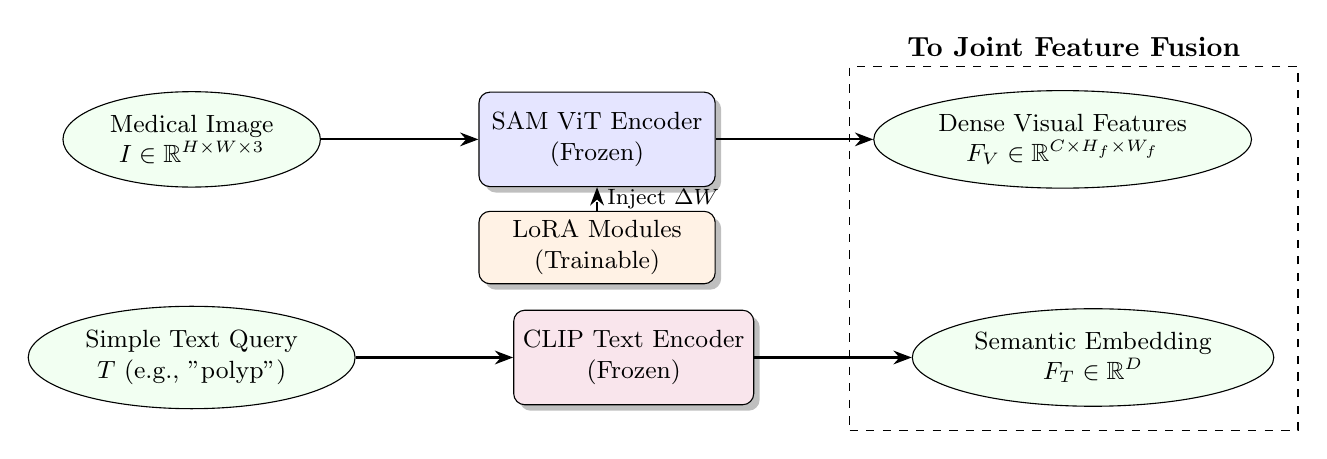
\begin{tikzpicture}[
    node distance=1.5cm and 2cm,
    box/.style={draw, rectangle, rounded corners, align=center, minimum width=3cm, minimum height=1.2cm, fill=blue!5, drop shadow, font=\small},
    data/.style={draw, ellipse, align=center, minimum width=2.5cm, minimum height=1cm, fill=green!5, font=\small},
    arrow/.style={-Stealth, thick}
]

% Visual Branch
\node[data] (img) {Medical Image\\$I \in \mathbb{R}^{H \times W \times 3}$};
\node[box, right=of img, fill=blue!10] (sam_enc) {SAM ViT Encoder\\(Frozen)};
\node[box, below=0.3cm of sam_enc, fill=orange!10, minimum height=0.8cm] (lora) {LoRA Modules\\(Trainable)};
\node[data, right=of sam_enc] (fv) {Dense Visual Features\\$F_V \in \mathbb{R}^{C \times H_f \times W_f}$};

% Text Branch
\node[data, below=1.5cm of img] (text) {Simple Text Query\\$T$ (e.g., "polyp")};
\node[box, right=of text, fill=purple!10] (clip_enc) {CLIP Text Encoder\\(Frozen)};
\node[data, right=of clip_enc] (ft) {Semantic Embedding\\$F_T \in \mathbb{R}^{D}$};

% Connections Visual
\draw[arrow] (img) -- (sam_enc);
\draw[arrow, dashed] (lora) -- (sam_enc) node[midway, right, font=\footnotesize] {Inject $\Delta W$};
\draw[arrow] (sam_enc) -- (fv);

% Connections Text
\draw[arrow] (text) -- (clip_enc);
\draw[arrow] (clip_enc) -- (ft);

% Grouping Box for the next stage
\node[draw, rectangle, dashed, fit=(fv) (ft), inner sep=0.3cm, label=above:\textbf{To Joint Feature Fusion}] (fusion_box) {};

\end{tikzpicture}%
}
\caption{The Cross-Modal Feature Extraction pipeline of CMA-SAM. The visual branch employs a SAM ViT encoder adapted via parameter-efficient LoRA modules to extract dense visual features $F_V$. Simultaneously, the text branch utilizes a frozen CLIP text encoder to extract a global semantic embedding $F_T$ from simple text queries.}
\label{fig:feature_extraction}
\end{figure}

\subsection{Joint Feature Fusion via Bidirectional Cross-Attention}

\subsubsection{Cross-Modal Alignment Formulation}
To deeply entangle the continuous semantic embeddings extracted by CLIP with the dense visual features encoded by SAM, we introduce a bidirectional cross-attention mechanism. Let $F_I \in \mathbb{R}^{C \times H \times W}$ denote the visual feature map and $F_T \in \mathbb{R}^{L \times D}$ denote the sequence of $L$ text token embeddings. We first flatten the spatial dimensions of the visual features to obtain a sequence of visual tokens $X_V \in \mathbb{R}^{N \times C}$, where $N = H \times W$. The text embeddings are linearly projected to match the visual channel dimension, yielding $X_T \in \mathbb{R}^{L \times C}$.

Standard multi-modal fusion techniques often rely on simple channel-wise concatenation or Hadamard product-based projections \cite{lin2023multi}. However, these operations fail to capture complex, long-range dependencies between specific textual concepts and localized visual regions. To address this, our bidirectional cross-attention explicitly models both Text-to-Vision (T2V) and Vision-to-Text (V2T) interactions \cite{wang2024sam}.

For the T2V attention, the visual tokens act as queries, while the text tokens serve as keys and values:
\begin{equation}
    Q_V = X_V W_{Q_V}, \quad K_T = X_T W_{K_T}, \quad V_T = X_T W_{V_T}
\end{equation}
\begin{equation}
    A_{T \to V} = \text{Softmax}\left(\frac{Q_V K_T^\top}{\sqrt{d}}\right) V_T
\end{equation}
where $W_{Q_V}, W_{K_T}, W_{V_T} \in \mathbb{R}^{C \times d}$ are learnable projection matrices, and $d$ is the hidden dimension. The resulting context matrix $A_{T \to V} \in \mathbb{R}^{N \times d}$ represents the semantic information injected into each visual token.

Conversely, the V2T attention updates the text representation with local structural context from the image:
\begin{equation}
    Q_T = X_T W_{Q_T}, \quad K_V = X_V W_{K_V}, \quad V_V = X_V W_{V_V}
\end{equation}
\begin{equation}
    A_{V \to T} = \text{Softmax}\left(\frac{Q_T K_V^\top}{\sqrt{d}}\right) V_V
\end{equation}

The updated visual and textual tokens are then computed using residual connections and a Feed-Forward Network (FFN):
\begin{align}
    \tilde{X}_V &= \text{LayerNorm}(X_V + \text{FFN}(A_{T \to V} W_{O_V})) \\
    \tilde{X}_T &= \text{LayerNorm}(X_T + \text{FFN}(A_{V \to T} W_{O_T}))
\end{align}
where $W_{O_V}$ and $W_{O_T}$ are output projection weights. Finally, the enriched visual tokens $\tilde{X}_V$ are reshaped back to the original spatial dimensions to form the continuous cross-modal representation $M \in \mathbb{R}^{C \times H \times W}$. This deeply coupled representation ensures that the visual features are heavily conditioned on the semantic target, providing a highly discriminative foundation for the subsequent anchor generation phase.

\subsubsection{Semantic Filtering and Background Suppression}
The bidirectional cross-attention mechanism inherently acts as a multi-modal information bottleneck \cite{wang2023visual}. In heterogeneous medical images, such as noisy ultrasound scans or diffuse MRI slices, the raw visual features $F_I$ often contain high-contrast background noise and modality-specific artifacts that can mislead downstream segmentation modules \cite{lan2024proxyclip}. 

By computing the dense affinity matrix $\frac{Q_V K_T^\top}{\sqrt{d}}$, the T2V attention assigns high activation weights exclusively to visual tokens that exhibit strong semantic correspondence with the text prompt. Consequently, this operation sharply highlights the target lesion while aggressively attenuating irrelevant anatomical structures. 

\begin{figure}[htbp]
\centering
\fitwidth{%
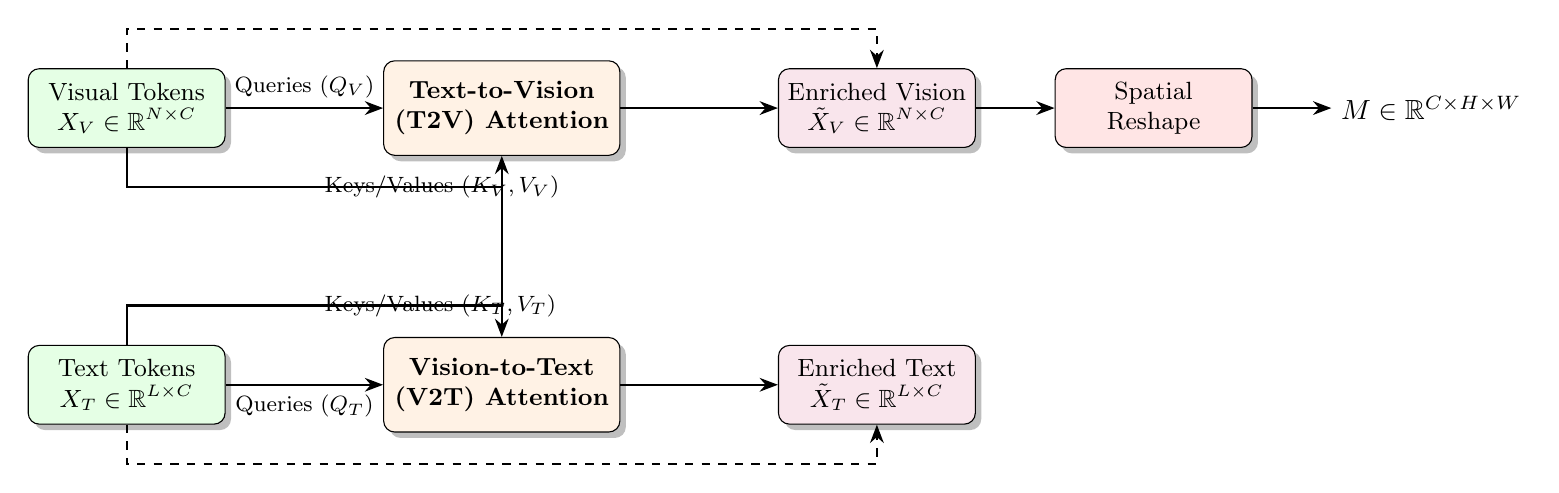
\begin{tikzpicture}[
    node distance=1.5cm and 2cm,
    box/.style={draw, rectangle, rounded corners, align=center, minimum width=2.5cm, minimum height=1cm, fill=blue!5, drop shadow, font=\small},
    attnbox/.style={draw, rectangle, rounded corners, align=center, minimum width=3cm, minimum height=1.2cm, fill=orange!10, drop shadow, font=\small\bfseries},
    arrow/.style={-Stealth, thick},
    label/.style={font=\footnotesize}
]

% Input Nodes
\node[box, fill=green!10] (vis_in) {Visual Tokens\\$X_V \in \mathbb{R}^{N \times C}$};
\node[box, fill=green!10, below=2.5cm of vis_in] (txt_in) {Text Tokens\\$X_T \in \mathbb{R}^{L \times C}$};

% Attention Blocks
\node[attnbox, right=of vis_in] (t2v) {Text-to-Vision\\(T2V) Attention};
\node[attnbox, right=of txt_in] (v2t) {Vision-to-Text\\(V2T) Attention};

% Output Nodes
\node[box, fill=purple!10, right=of t2v] (vis_out) {Enriched Vision\\$\tilde{X}_V \in \mathbb{R}^{N \times C}$};
\node[box, fill=purple!10, right=of v2t] (txt_out) {Enriched Text\\$\tilde{X}_T \in \mathbb{R}^{L \times C}$};

% Reshape Node
\node[box, fill=red!10, right=1cm of vis_out] (reshape) {Spatial\\Reshape};
\node[right=1cm of reshape, font=\bfseries] (final_M) {$M \in \mathbb{R}^{C \times H \times W}$};

% Arrows for T2V
\draw[arrow] (vis_in) -- node[above, label] {Queries ($Q_V$)} (t2v);
\draw[arrow] (txt_in.north) -- ++(0,0.5) -| node[near start, right, label] {Keys/Values ($K_T, V_T$)} (t2v.south);

% Arrows for V2T
\draw[arrow] (txt_in) -- node[below, label] {Queries ($Q_T$)} (v2t);
\draw[arrow] (vis_in.south) -- ++(0,-0.5) -| node[near start, right, label] {Keys/Values ($K_V, V_V$)} (v2t.north);

% Output Arrows
\draw[arrow] (t2v) -- (vis_out);
\draw[arrow] (v2t) -- (txt_out);

% Reshape Arrows
\draw[arrow] (vis_out) -- (reshape);
\draw[arrow] (reshape) -- (final_M);

% Residual connections
\draw[arrow, dashed] (vis_in.north) -- ++(0,0.5) -| (vis_out.north);
\draw[arrow, dashed] (txt_in.south) -- ++(0,-0.5) -| (txt_out.south);

\end{tikzpicture}%
}
\caption{Architecture of the Bidirectional Cross-Attention module. The mechanism explicitly models both Text-to-Vision (T2V) and Vision-to-Text (V2T) interactions, acting as a semantic filter to generate the highly discriminative cross-modal representation $M$.}
\label{fig:cross_attention}
\end{figure}

As illustrated in Figure \ref{fig:cross_attention}, the V2T attention complements this filtering process by dynamically updating the text embeddings based on the visual context. If a simple class name (e.g., ``polyp'') is provided, the V2T attention enriches this sparse semantic query with specific morphological features present in the image, effectively creating a tailored, image-conditioned prompt. This dual-filtering mechanism ensures that the resulting cross-modal representation $M$ is unimodal and highly localized, providing a clean spatial prior that prevents the subsequent Autonomous Anchor Generation (AAG) module from regressing spurious coordinates outside the region of interest.

\subsection{Autonomous Anchor Generation (AAG) Module}

The core innovation of the CMA-SAM framework is the Autonomous Anchor Generation (AAG) module. This module bridges the gap between the continuous, high-dimensional semantic representations produced by Vision-Language Models and the discrete, coordinate-driven prompt encoder native to the Segment Anything Model (SAM) \cite{kirillov2023segment}. Given the fused cross-modal feature map $M \in \mathbb{R}^{C \times H \times W}$ obtained from the bidirectional cross-attention mechanism, the AAG module explicitly regresses a set of discrete point prompts $P = \{(x_k, y_k)\}_{k=1}^K$ and a global bounding box $B = (x_{\min}, y_{\min}, x_{\max}, y_{\max})$.

\subsubsection{Differentiable Point Prompt Regression via Spatial Softmax}

Unlike heuristic-based self-prompting methods that rely on non-differentiable visual saliency thresholding or edge detection \cite{xie2025self, chen2024un}, the AAG module employs a fully differentiable Spatial Softmax operation. This ensures that the anchor generation process can be optimized end-to-end via backpropagation.

First, the fused feature map $M$ is processed by a lightweight convolutional block $f_{\text{conv}}$ (comprising a $3 \times 3$ convolution, Batch Normalization, and a ReLU activation, followed by a $1 \times 1$ convolution) to project the channel dimension from $C$ to $K$, where $K$ is the desired number of point prompts. To prevent logit saturation and enforce the bounded activation premise required for strictly positive Spatial Softmax probabilities (Proposition \ref{prop:nonzero_gradients}), we apply a scaled hyperbolic tangent nonlinearity with cap $c = 3.0$, yielding $K$ bounded spatial activation maps $S \in [-c, c]^{K \times H \times W}$:
\begin{equation}
    S = c \tanh\!\big(f_{\text{conv}}(M)\big)
\end{equation}

For the $k$-th activation map $S_k \in \mathbb{R}^{H \times W}$, we compute a 2D probability distribution $p_k$ over the spatial grid using the Spatial Softmax function. The probability of the target point being located at spatial coordinates $(i, j)$ is given by:
\begin{equation}
    p_{k, i, j} = \frac{\exp(S_{k, i, j} / \tau)}{\sum_{u=1}^{W} \sum_{v=1}^{H} \exp(S_{k, v, u} / \tau)}
\end{equation}
where $\tau$ is the temperature parameter. The discrete coordinates $(x_k, y_k)$ for the $k$-th point prompt are then obtained by computing the expected value of the spatial coordinates over this probability distribution:
\begin{equation}
    (x_k, y_k) = \left( \sum_{i=1}^{W} \sum_{j=1}^{H} i \cdot p_{k, i, j}, \quad \sum_{i=1}^{W} \sum_{j=1}^{H} j \cdot p_{k, i, j} \right)
\end{equation}
This expectation formulation provides a continuous and differentiable approximation of the discrete $\arg\max$ operator, allowing the gradients from the SAM mask decoder to flow directly back into the cross-modal fusion layers.

\subsubsection{Dynamic Temperature Scaling for Morphological Adaptation}

The temperature parameter $\tau$ plays a critical role in modulating the sharpness of the spatial probability distribution $p_k$. If $\tau \to \infty$, the distribution approaches a uniform state, leading to coordinates that collapse toward the center of the image. Conversely, if $\tau \to 0$, the operation approximates a hard $\arg\max$, which yields sharp localizations but suffers from vanishing gradients during training.

Medical targets exhibit extreme morphological variance, ranging from highly diffuse and poorly demarcated polyps in endoscopy \cite{jha2020kvasir} to sharply defined melanomas in dermatology \cite{codella2018skin}. Utilizing a fixed temperature often results in overly smooth attribution maps that fail to isolate salient target regions \cite{wang2023visual}. To accommodate this variance, we formulate $\tau$ as a dynamically learnable parameter optimized alongside the network weights:
\begin{equation}
    \tau = \text{Softplus}(w_\tau) + \epsilon = \ln(1 + \exp(w_\tau)) + \epsilon
\end{equation}
where $w_\tau$ is a learnable scalar initialized to correspond to $\tau = 0.1$, and $\epsilon = 10^{-4}$ is a small constant to prevent division by zero. This dynamic scaling allows the AAG module to adaptively sharpen the distribution for well-defined structures and soften it to capture broader regional context for diffuse lesions.

\subsubsection{Global Bounding Box Regression}

While point prompts provide high-frequency local guidance for specific tissue sub-regions, relying solely on points can lead to the erroneous segmentation of disjoint background regions that share similar textural features with the target. To mitigate this, the AAG module simultaneously regresses a global bounding box to serve as a strict macroscopic spatial constraint, a strategy proven effective in medical adaptations of SAM \cite{dai2024samaug}.

The bounding box regression branch applies Global Average Pooling (GAP) to the fused feature map $M$ to extract a holistic semantic descriptor $z \in \mathbb{R}^C$:
\begin{equation}
    z = \frac{1}{H \times W} \sum_{i=1}^{W} \sum_{j=1}^{H} M_{:, j, i}
\end{equation}
This vector $z$ is normalized via Layer Normalization \cite{ba2016layer} and passed through a two-layer ReLU Multi-Layer Perceptron (MLP) followed by a Sigmoid activation $\sigma(\cdot)$ that predicts normalized center-size parameters $(\hat{c}_x, \hat{c}_y, \hat{w}, \hat{h}) = \sigma(\text{MLP}(\text{LN}(z))) \in (0, 1)^4$, which are deterministically mapped to valid ordered box corners in $[0, 1]^4$:
\begin{equation}
    B = \big(\text{clamp}(\hat{c}_x - \tfrac{\hat{w}}{2}, 0, 1),\; \text{clamp}(\hat{c}_y - \tfrac{\hat{h}}{2}, 0, 1),\; \text{clamp}(\hat{c}_x + \tfrac{\hat{w}}{2}, 0, 1),\; \text{clamp}(\hat{c}_y + \tfrac{\hat{h}}{2}, 0, 1)\big) = (x_{\min}, y_{\min}, x_{\max}, y_{\max})
\end{equation}
The generated bounding box $B$ and the set of point prompts $P$ are subsequently denormalized to the original image dimensions and fed into SAM's native prompt encoder. 

The complete forward pass of the AAG module is summarized in Algorithm \ref{alg:aag_forward}, and its architectural flow is illustrated in Figure \ref{fig:aag_architecture}.

\begin{algorithm}[htbp]
\caption{Autonomous Anchor Generation (AAG) Forward Pass}
\label{alg:aag_forward}
\begin{algorithmic}[1]
\Require Fused cross-modal feature map $M \in \mathbb{R}^{C \times H \times W}$, Number of points $K$
\Ensure Point prompts $P = \{(x_k, y_k)\}_{k=1}^K$, Bounding box $B$
\State \textbf{Initialize:} Learnable temperature weight $w_\tau$
\State $\tau \gets \ln(1 + \exp(w_\tau)) + 10^{-4}$ \Comment{Compute dynamic temperature}
\State $S \gets c \tanh(f_{\text{conv}}(M))$ \Comment{Bounded activation maps, $S \in [-c, c]^{K \times H \times W}$}
\State $P \gets \emptyset$
\For{$k = 1$ to $K$}
    \State $p_k \gets \text{SpatialSoftmax}(S_k, \tau)$ \Comment{Compute 2D probability map}
    \State $x_k \gets \sum_{i=1}^{W} \sum_{j=1}^{H} i \cdot p_{k, i, j}$ \Comment{Expected X coordinate}
    \State $y_k \gets \sum_{i=1}^{W} \sum_{j=1}^{H} j \cdot p_{k, i, j}$ \Comment{Expected Y coordinate}
    \State $P \gets P \cup \{(x_k, y_k)\}$
\EndFor
\State $z \gets \text{GAP}(M)$ \Comment{Global Average Pooling for box regression}
\State $B \gets \sigma(\text{MLP}(z))$ \Comment{Regress normalized bounding box coordinates}
\State \Return $P, B$
\end{algorithmic}
\end{algorithm}

\begin{figure}[htbp]
\centering
\fitwidth{%
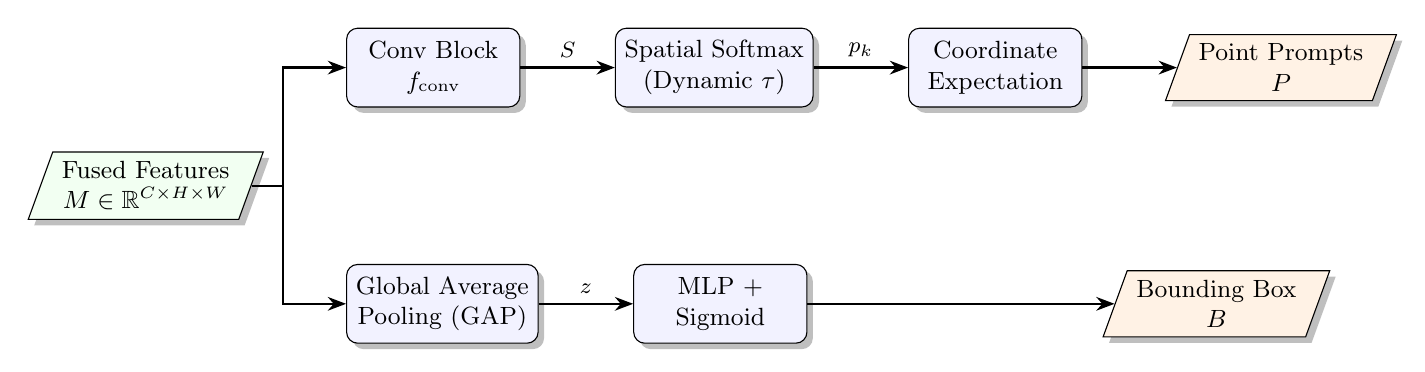
\begin{tikzpicture}[
    node distance=0.8cm and 1.2cm,
    box/.style={draw, rectangle, rounded corners, align=center, minimum width=2.2cm, minimum height=1cm, fill=blue!5, drop shadow, font=\small},
    io/.style={draw, trapezium, trapezium left angle=70, trapezium right angle=110, align=center, fill=green!5, drop shadow, font=\small},
    arrow/.style={-Stealth, thick}
]

% Input
\node[io] (input) {Fused Features\\$M \in \mathbb{R}^{C \times H \times W}$};

% Point Branch (Top)
\node[box, right=of input, yshift=1.5cm] (conv) {Conv Block\\$f_{\text{conv}}$};
\node[box, right=of conv] (softmax) {Spatial Softmax\\(Dynamic $\tau$)};
\node[box, right=of softmax] (expectation) {Coordinate\\Expectation};
\node[io, right=of expectation, fill=orange!10] (points) {Point Prompts\\$P$};

% Box Branch (Bottom)
\node[box, right=of input, yshift=-1.5cm] (gap) {Global Average\\Pooling (GAP)};
\node[box, right=of gap] (mlp) {MLP +\\Sigmoid};
\node[io, right=of mlp, fill=orange!10, xshift=2.7cm] (box) {Bounding Box\\$B$};

% Connections
\draw[arrow] (input.east) -- ++(0.4,0) |- (conv.west);
\draw[arrow] (input.east) -- ++(0.4,0) |- (gap.west);

\draw[arrow] (conv.east) -- node[above, font=\footnotesize] {$S$} (softmax.west);
\draw[arrow] (softmax.east) -- node[above, font=\footnotesize] {$p_k$} (expectation.west);
\draw[arrow] (expectation.east) -- (points.west);

\draw[arrow] (gap.east) -- node[above, font=\footnotesize] {$z$} (mlp.west);
\draw[arrow] (mlp.east) -- (box.west);

\end{tikzpicture}%
}
\caption{Internal architecture of the Autonomous Anchor Generation (AAG) module. The module processes the fused cross-modal features through two parallel, fully differentiable branches to regress local point prompts and a global bounding box.}
\label{fig:aag_architecture}
\end{figure}

\subsection{Mask Decoding and End-to-End Learning Mechanism}

\subsubsection{Integration with SAM's Native Prompt Encoder}
Following the autonomous regression of discrete geometric coordinates by the Autonomous Anchor Generation (AAG) module, the generated point set $P = \{(x_i, y_i)\}_{i=1}^K$ and the bounding box $B = (x_{\min}, y_{\min}, x_{\max}, y_{\max})$ are directly injected into the native prompt encoder of the Segment Anything Model (SAM) \cite{kirillov2023segment}. SAM's prompt encoder maps these discrete spatial coordinates into high-dimensional sparse embeddings. Specifically, each point $(x_i, y_i)$ is embedded as a sum of a positional encoding and a learned state embedding indicating whether the point represents foreground or background. The bounding box $B$ is embedded using an analogous positional encoding of its top-left and bottom-right corners.

By feeding these autonomously generated anchors into the frozen prompt encoder, CMA-SAM explicitly decouples the semantic localization task from the boundary delineation task. The AAG module, conditioned on the cross-modal features, assumes full responsibility for identifying the target's macroscopic location and internal structure. Consequently, SAM's highly optimized mask decoder is relieved of the burden of resolving global semantics and can focus exclusively on high-frequency boundary refinement using the dense image embeddings $F_I$ and the sparse prompt embeddings. This architectural decoupling effectively circumvents the spatial hallucinations commonly observed in direct dense decoding paradigms.

\subsubsection{Loss Functions and Mask-Derived Geometric Supervision}
To optimize CMA-SAM end-to-end without requiring any manual point or bounding-box annotations, we combine pixel-level mask supervision with zero-cost mask-derived geometric anchor supervision extracted directly from the ground-truth binary segmentation mask $Y \in \{0, 1\}^{H \times W}$. Because SAM's frozen prompt encoder maps normalized coordinates through high-frequency Fourier positional encodings, supervising $\hat{Y} \in [0, 1]^{H \times W}$ solely with pixel losses can exhibit oscillatory coordinate landscapes during early optimization. Extracting canonical interior point targets $P_{\text{gt}}(Y) = \{p_k^*\}_{k=1}^K \subset [0, 1]^2$ and the tightest foreground bounding box $B_{\text{gt}}(Y) \in [0, 1]^4$ directly from $Y$ provides clean, convex geometric guidance during training while leaving inference strictly dependent only on $(I, T)$. Specifically, $p_1^*$ is defined as the foreground centroid snapped to the nearest interior foreground pixel of $Y$, and for $K > 1$, the remaining $K - 1$ targets are obtained by partitioning foreground pixels into $K - 1$ ordered angular sectors around $p_1^*$ and snapping each sector's interior mean ($0.7\,\bar{q}_k + 0.3\,p_1^*$) to its closest foreground pixel; $B_{\text{gt}}(Y)$ encloses the foreground support of $Y$ with a $1.5\%$ margin.

The joint training objective $\mathcal{L}_{\text{total}}$ combines Dice loss \cite{milletari2016vnet}, Binary Cross-Entropy (BCE) loss, and the mask-derived anchor loss ($\lambda_{\text{dice}} = 1.0$, $\lambda_{\text{bce}} = 1.0$, $\lambda_{\text{anchor}} = 2.0$):
\begin{equation}
    \mathcal{L}_{\text{total}} = \lambda_{\text{dice}} \mathcal{L}_{\text{dice}}(Y, \hat{Y}) + \lambda_{\text{bce}} \mathcal{L}_{\text{bce}}(Y, \hat{Y}) + \lambda_{\text{anchor}} \mathcal{L}_{\text{anchor}}(\hat{P}, \hat{B}, Y)
\end{equation}
where $\hat{P}$ and $\hat{B}$ denote normalized predicted anchors, and the segmentation and geometric terms are given by:
\begin{equation}
    \mathcal{L}_{\text{dice}}(Y, \hat{Y}) = 1 - \frac{2 \sum_{i=1}^{H \times W} Y_i \hat{Y}_i + \epsilon}{\sum_{i=1}^{H \times W} Y_i + \sum_{i=1}^{H \times W} \hat{Y}_i + \epsilon}, \qquad
    \mathcal{L}_{\text{bce}}(Y, \hat{Y}) = - \frac{1}{H \times W} \sum_{i=1}^{H \times W} \left[ Y_i \log(\hat{Y}_i) + (1 - Y_i) \log(1 - \hat{Y}_i) \right]
\end{equation}
\begin{equation}
    \mathcal{L}_{\text{anchor}}(\hat{P}, \hat{B}, Y) = \frac{1}{K}\sum_{k=1}^{K} \ell_{\beta}(\hat{p}_k, p_k^*) + \ell_{\beta}(\hat{B}, B_{\text{gt}}(Y)) + 0.5\,\big(1 - \text{GIoU}(\hat{B}, B_{\text{gt}}(Y))\big)
\end{equation}
where $\ell_{\beta}$ denotes the Smooth-$L_1$ loss ($\beta = 0.02$) and $\epsilon = 10^{-5}$ prevents division by zero.

During training, gradients from both the mask decoder and $\mathcal{L}_{\text{anchor}}$ backpropagate jointly through the differentiable AAG module into the cross-modal fusion layers and SAM LoRA adapters. We optimize trainable parameters with AdamW \cite{loshchilov2017decoupled}, assigning zero weight decay to normalization parameters and the scalar temperature weight $w_\tau$ (with a $5\times$ learning-rate multiplier on $w_\tau$) so regularization never artificially drags $\tau$ toward a fixed value while the CLIP text encoder, SAM prompt encoder, and SAM mask decoder remain frozen.

\subsubsection{Inference and Final Algorithm}
During inference, the CMA-SAM framework operates in a fully autonomous, prompt-free manner from the user's perspective. Given a medical image and a simple text query (e.g., a basic anatomical class name), the model synthesizes the discrete geometric prompts internally and decodes the final segmentation mask in a single forward pass. 

This streamlined inference pipeline, detailed in Algorithm \ref{alg:cma_sam_inference}, drastically reduces computational latency. Unlike heavy hierarchical decoding adaptations \cite{cheng2024unleashing} that require extensive parameter updates to the decoder, or cascaded frameworks \cite{li2024clipsam} that sequentially process images through multiple disjoint foundation models, CMA-SAM leverages the native efficiency of SAM's geometric decoding. The lightweight nature of the AAG module ensures that the overhead introduced by the semantic-to-spatial translation is minimal, making CMA-SAM highly suitable for real-time clinical deployment.

\begin{algorithm}[htbp]
\caption{CMA-SAM End-to-End Inference Pipeline}
\label{alg:cma_sam_inference}
\begin{algorithmic}[1]
\Require Medical Image $I \in \mathbb{R}^{3 \times H_0 \times W_0}$, Simple Text Query $T$ (e.g., "polyp")
\Require Frozen CLIP Text Encoder $\mathcal{E}_{\text{text}}$, LoRA-adapted SAM Image Encoder $\mathcal{E}_{\text{img}}$
\Require Bidirectional Cross-Attention Fusion Module $\mathcal{F}$
\Require Autonomous Anchor Generation Module $\mathcal{A}$
\Require Frozen SAM Prompt Encoder $\mathcal{P}$, Frozen SAM Mask Decoder $\mathcal{D}$
\Ensure Predicted Segmentation Mask $\hat{Y} \in \{0, 1\}^{H_0 \times W_0}$

\State \textbf{Step 1: Cross-Modal Feature Extraction}
\State $F_T \gets \mathcal{E}_{\text{text}}(T)$ \Comment{Extract semantic text embedding}
\State $F_I \gets \mathcal{E}_{\text{img}}(I)$ \Comment{Extract dense visual features}

\State \textbf{Step 2: Joint Feature Fusion}
\State $M \gets \mathcal{F}(F_I, F_T)$ \Comment{Compute cross-modal representation via bidirectional attention}

\State \textbf{Step 3: Autonomous Anchor Generation}
\State $S \gets \text{ConvHead}(M)$ \Comment{Generate $K$ point activation maps}
\State $P \gets \text{SpatialSoftmax}(S, \tau)$ \Comment{Regress discrete point coordinates $P = \{(x_i, y_i)\}_{i=1}^K$}
\State $B \gets \sigma(\text{MLP}(\text{GAP}(M)))$ \Comment{Regress global bounding box $B$}

\State \textbf{Step 4: Mask Decoding}
\State $E_{\text{sparse}} \gets \mathcal{P}(P, B)$ \Comment{Encode discrete anchors into sparse embeddings}
\State $\hat{Y}_{\text{prob}} \gets \mathcal{D}(F_I, E_{\text{sparse}})$ \Comment{Decode mask probabilities using dense and sparse embeddings}
\State $\hat{Y} \gets \text{Binarize}(\hat{Y}_{\text{prob}}, \text{threshold}=0.5)$ \Comment{Generate final binary mask}

\State \Return $\hat{Y}$
\end{algorithmic}
\end{algorithm}
\section{Theoretical Analysis}

\subsection{Gradient Flow and Differentiability of the Autonomous Anchor Generation}

To rigorously establish the end-to-end learning capability of the Cross-Modal Anchor Segment Anything Model (CMA-SAM), we must formally analyze the differentiability of the Autonomous Anchor Generation (AAG) module. Unlike heuristic-based self-prompting methods that rely on non-differentiable hard \(\arg\max\) operations or thresholding \cite{xie2025self, chen2024un}, our AAG module employs an expectation-based Spatial Softmax formulation. This section derives the Jacobian of the generated coordinates, proves the guarantee of non-zero gradients, and establishes the stability conditions provided by the dynamic temperature parameter \(\tau\).

Let \(S \in \mathbb{R}^{W \times H}\) denote the spatial activation map for a single point prompt (omitting the point index \(k\) for notational simplicity). The spatial probability distribution is defined as \(p_{i,j} = \frac{\exp(S_{i,j}/\tau)}{Z}\), where \(Z = \sum_{u=1}^W \sum_{v=1}^H \exp(S_{u,v}/\tau)\). The expected coordinates are given by \(x = \sum_{i=1}^W \sum_{j=1}^H i \cdot p_{i,j}\) and \(y = \sum_{i=1}^W \sum_{j=1}^H j \cdot p_{i,j}\).

\begin{theorem}[Jacobian of the Expected Coordinates]
\label{thm:jacobian_spatial_softmax}
The partial derivatives of the expected spatial coordinates \((x, y)\) with respect to the input activation map \(S\) and the dynamic temperature parameter \(\tau\) are given by:
\begin{align}
    \frac{\partial x}{\partial S_{m,n}} &= \frac{1}{\tau} p_{m,n} (m - x) \label{eq:grad_x_S} \\
    \frac{\partial y}{\partial S_{m,n}} &= \frac{1}{\tau} p_{m,n} (n - y) \label{eq:grad_y_S} \\
    \frac{\partial x}{\partial \tau} &= -\frac{1}{\tau^2} \mathrm{Cov}_{p}(X, S) \label{eq:grad_x_tau}
\end{align}
where \(\mathrm{Cov}_{p}(X, S) = \sum_{i,j} i \cdot p_{i,j} (S_{i,j} - \bar{S})\) is the spatial covariance between the coordinate grid \(X\) and the activation map \(S\), with \(\bar{S} = \sum_{u,v} p_{u,v} S_{u,v}\).
\end{theorem}

\begin{proof}
We first derive the derivative of the probability \(p_{i,j}\) with respect to a specific activation \(S_{m,n}\). Using the quotient rule:
\begin{equation}
    \frac{\partial p_{i,j}}{\partial S_{m,n}} = \frac{1}{\tau} p_{i,j} (\delta_{i,m}\delta_{j,n} - p_{m,n})
\end{equation}
where \(\delta\) is the Kronecker delta. Applying the chain rule to the expected coordinate \(x\):
\begin{align}
    \frac{\partial x}{\partial S_{m,n}} &= \sum_{i=1}^W \sum_{j=1}^H i \frac{\partial p_{i,j}}{\partial S_{m,n}} \nonumber \\
    &= \frac{1}{\tau} \sum_{i=1}^W \sum_{j=1}^H i \cdot p_{i,j} (\delta_{i,m}\delta_{j,n} - p_{m,n}) \nonumber \\
    &= \frac{1}{\tau} \left( m \cdot p_{m,n} - p_{m,n} \sum_{i=1}^W \sum_{j=1}^H i \cdot p_{i,j} \right) \nonumber \\
    &= \frac{1}{\tau} p_{m,n} (m - x)
\end{align}
The derivation for \(\frac{\partial y}{\partial S_{m,n}}\) follows symmetrically. For the temperature parameter \(\tau\), the derivative of the probability is:
\begin{equation}
    \frac{\partial p_{i,j}}{\partial \tau} = -\frac{1}{\tau^2} p_{i,j} (S_{i,j} - \bar{S})
\end{equation}
Substituting this into the expectation yields:
\begin{equation}
    \frac{\partial x}{\partial \tau} = -\frac{1}{\tau^2} \sum_{i=1}^W \sum_{j=1}^H i \cdot p_{i,j} (S_{i,j} - \bar{S}) = -\frac{1}{\tau^2} \mathrm{Cov}_{p}(X, S)
\end{equation}
which completes the proof.
\end{proof}

\begin{proposition}[Guarantee of Non-Zero Gradients]
\label{prop:nonzero_gradients}
Unlike the hard \(\arg\max\) operation utilized in discrete anchor generation baselines \cite{xie2025self, chen2024un}, the expectation-based Spatial Softmax guarantees non-zero gradients almost everywhere, enabling continuous gradient flow from the SAM mask decoder \cite{kirillov2023segment} to the cross-modal fusion layers.
\end{proposition}

\begin{proof}
The hard \(\arg\max\) function can be formulated as the limit of the Spatial Softmax as \(\tau \to 0^+\). In this limit, the probability distribution converges to a Dirac delta function centered at the maximum activation. Consequently, the derivative \(\frac{\partial x_{\arg\max}}{\partial S_{m,n}} = 0\) almost everywhere, completely halting backpropagation. 

Conversely, for any finite \(\tau > 0\) and bounded activation \(S_{m,n} \in \mathbb{R}\), the exponential function ensures that \(p_{m,n} > 0\) strictly. From Equation \ref{eq:grad_x_S}, the gradient \(\frac{\partial x}{\partial S_{m,n}} = 0\) if and only if \(m = x\). Since \(x\) is a continuous expectation over the discrete grid \(\{1, \dots, W\}\), the condition \(m = x\) can hold for at most one grid index \(m\). For all other \(W-1\) indices along the x-axis, \(m - x \neq 0\), ensuring that \(\nabla_S x \neq \mathbf{0}\). Thus, gradients flow continuously to the preceding layers.
\end{proof}

\begin{figure}[htbp]
\centering
\fitwidth{%
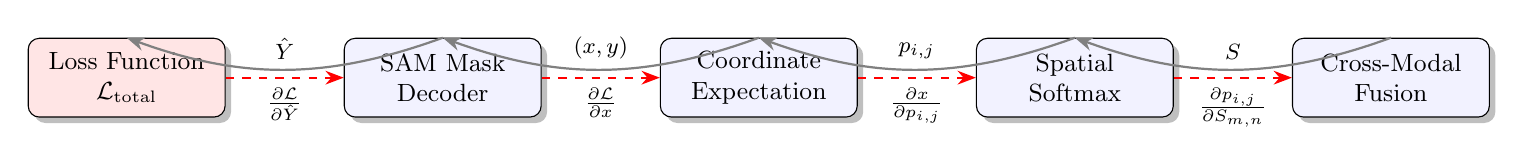
\begin{tikzpicture}[
    node distance=1.5cm and 1.5cm,
    box/.style={draw, rectangle, rounded corners, align=center, minimum width=2.5cm, minimum height=1cm, fill=blue!5, drop shadow, font=\small},
    grad/.style={-Stealth, thick, dashed, red},
    forward/.style={-Stealth, thick, gray}
]

% Nodes
\node[box, fill=red!10] (loss) {Loss Function\\$\mathcal{L}_{\text{total}}$};
\node[box, right=of loss] (decoder) {SAM Mask\\Decoder};
\node[box, right=of decoder] (expectation) {Coordinate\\Expectation};
\node[box, right=of expectation] (softmax) {Spatial\\Softmax};
\node[box, right=of softmax] (fusion) {Cross-Modal\\Fusion};

% Forward paths (background)
\draw[forward] (fusion.north) to[bend left=20] node[above, font=\footnotesize, text=black] {$S$} (softmax.north);
\draw[forward] (softmax.north) to[bend left=20] node[above, font=\footnotesize, text=black] {$p_{i,j}$} (expectation.north);
\draw[forward] (expectation.north) to[bend left=20] node[above, font=\footnotesize, text=black] {$(x,y)$} (decoder.north);
\draw[forward] (decoder.north) to[bend left=20] node[above, font=\footnotesize, text=black] {$\hat{Y}$} (loss.north);

% Backward paths (foreground)
\draw[grad] (loss) -- node[below, font=\footnotesize, text=black] {$\frac{\partial \mathcal{L}}{\partial \hat{Y}}$} (decoder);
\draw[grad] (decoder) -- node[below, font=\footnotesize, text=black] {$\frac{\partial \mathcal{L}}{\partial x}$} (expectation);
\draw[grad] (expectation) -- node[below, font=\footnotesize, text=black] {$\frac{\partial x}{\partial p_{i,j}}$} (softmax);
\draw[grad] (softmax) -- node[below, font=\footnotesize, text=black] {$\frac{\partial p_{i,j}}{\partial S_{m,n}}$} (fusion);

\end{tikzpicture}%
}
\caption{Conceptual diagram of the continuous gradient flow during backpropagation. The differentiable expectation mechanism ensures that error signals from the SAM mask decoder \cite{kirillov2023segment} successfully traverse the AAG module to update the cross-modal fusion representations.}
\label{fig:gradient_flow}
\end{figure}

While Proposition \ref{prop:nonzero_gradients} establishes the existence of gradients, the magnitude of these gradients is highly sensitive to the temperature \(\tau\). If \(\tau\) is too small, gradients may explode; if \(\tau\) is too large, they may vanish. To ensure stable end-to-end backpropagation, CMA-SAM parameterizes the temperature dynamically as \(\tau = \ln(1 + \exp(w_\tau)) + \epsilon\).

\begin{theorem}[Gradient Stability Bounds]
\label{thm:gradient_stability}
Given the dynamic temperature formulation \(\tau = \ln(1 + \exp(w_\tau)) + \epsilon\) with a strictly positive constant \(\epsilon > 0\), the gradient of the expected coordinates with respect to the activation map is strictly bounded, preventing gradient explosion. Furthermore, the gradient of the temperature parameter itself is bounded, ensuring stable optimization.
\end{theorem}

\begin{proof}
To prove the prevention of gradient explosion, we bound the infinity norm of the Jacobian \(\nabla_S x\). From Equation \ref{eq:grad_x_S}, we have:
\begin{equation}
    \left| \frac{\partial x}{\partial S_{m,n}} \right| = \left| \frac{1}{\tau} p_{m,n} (m - x) \right|
\end{equation}
Since \(p_{m,n} \in (0, 1)\) is a valid probability and both \(m\) and \(x\) are constrained within the image width \([1, W]\), the maximum spatial distance is \(|m - x| < W\). Furthermore, by definition, \(\tau = \ln(1 + \exp(w_\tau)) + \epsilon \ge \epsilon\). Therefore:
\begin{equation}
    \left\| \nabla_S x \right\|_\infty < \frac{1}{\epsilon} \cdot 1 \cdot W = \frac{W}{\epsilon}
\end{equation}
Because \(W\) is finite and \(\epsilon > 0\), the gradient is strictly bounded from above, mathematically precluding gradient explosion even as the network attempts to sharpen the probability distribution (\(w_\tau \to -\infty\)).

Next, we analyze the stability of updating the learnable weight \(w_\tau\). By the chain rule:
\begin{equation}
    \frac{\partial \mathcal{L}}{\partial w_\tau} = \frac{\partial \mathcal{L}}{\partial x} \frac{\partial x}{\partial \tau} \frac{\partial \tau}{\partial w_\tau}
\end{equation}
The derivative of the Softplus function is the standard Sigmoid function:
\begin{equation}
    \frac{\partial \tau}{\partial w_\tau} = \frac{\exp(w_\tau)}{1 + \exp(w_\tau)} = \sigma(w_\tau) \in (0, 1)
\end{equation}
Since \(\sigma(w_\tau)\) is strictly bounded between 0 and 1, and \(\frac{\partial x}{\partial \tau}\) is bounded by the spatial covariance (Equation \ref{eq:grad_x_tau}), the gradient \(\frac{\partial \mathcal{L}}{\partial w_\tau}\) remains stable. This allows the network to dynamically adapt \(\tau\) to the morphological variance of the medical targets without destabilizing the broader cross-modal fusion training dynamics.
\end{proof}

\subsection{Error Bounds on Cross-Modal Anchor Localization}

To rigorously evaluate the robustness of the Autonomous Anchor Generation (AAG) module, we establish theoretical upper bounds on the Anchor Localization Error (ALE) introduced during the semantic-to-spatial translation phase. In multi-modal architectures, the translation from the continuous semantic space of Vision-Language Models (VLMs) to the spatial domain of Vision Foundation Models is inherently susceptible to modality-gap noise. We demonstrate that our expectation-based formulation strictly constrains this error, preventing the catastrophic failures observed in sequential cascaded pipelines \cite{aleem2024test, li2024clipsam}.

\subsubsection{Modality-Gap Noise Model and Error Propagation}

Let $\mathcal{X} \subset \mathbb{R}^2$ denote the continuous spatial domain of the image. We model the cross-modal feature map generated by the Joint Feature Fusion module as a true underlying spatial signal corrupted by bounded noise.

\begin{definition}[Modality-Gap Noise]
Let $S_k(x)$ be the true, uncorrupted spatial activation map for the $k$-th point prompt, perfectly reflecting the semantic alignment between the image and the text query. The observed activation map $\tilde{S}_k(x)$ is defined as:
\begin{equation}
    \tilde{S}_k(x) = S_k(x) + \epsilon(x)
\end{equation}
where $\epsilon(x)$ represents the modality-gap noise. We assume this noise is uniformly bounded such that $\sup_{x \in \mathcal{X}} |\epsilon(x)| \le \delta$ for some $\delta > 0$.
\end{definition}

In the AAG module, the expected spatial coordinate for the $k$-th point prompt under the true signal is $\mu_k = \mathbb{E}_{p_k}[x]$, where $p_k(x; \tau) \propto \exp(S_k(x)/\tau)$. Under the noisy signal, the perturbed coordinate is $\tilde{\mu}_k = \mathbb{E}_{\tilde{p}_k}[x]$. The Anchor Localization Error (ALE) is given by $\|\tilde{\mu}_k - \mu_k\|_2$.

\begin{theorem}[Anchor Localization Error Bound]
\label{thm:ale_bound}
Given a noise bound $\delta$ and a dynamic temperature parameter $\tau$, the Anchor Localization Error for the $k$-th point prompt is strictly bounded by:
\begin{equation}
    \|\tilde{\mu}_k - \mu_k\|_2 \le \frac{\delta}{\tau} \sup_{t \in [0,1]} \sqrt{\mathrm{Tr}(\Sigma_{k, t})}
\end{equation}
where $\Sigma_{k, t}$ is the spatial covariance matrix of the distribution $p_{k, t}$ induced by the interpolated logits $S_k(x) + t\epsilon(x)$.
\end{theorem}

\begin{proof}
Let $f(t) = \mathbb{E}_{p_{k, t}}[x]$ be the expected coordinate parameterized by $t \in [0, 1]$, where $p_{k, t}(x) \propto \exp((S_k(x) + t\epsilon(x))/\tau)$. By the Fundamental Theorem of Calculus, $\tilde{\mu}_k - \mu_k = \int_{0}^{1} f'(t) dt$. 

The derivative of the expectation of the Spatial Softmax with respect to $t$ is given by the scaled covariance between the spatial coordinates and the perturbation:
\begin{equation}
    f'(t) = \frac{1}{\tau} \mathrm{Cov}_{p_{k, t}}(x, \epsilon(x)) = \frac{1}{\tau} \mathbb{E}_{p_{k, t}} \left[ (x - f(t)) (\epsilon(x) - \bar{\epsilon}_t) \right]
\end{equation}
where $\bar{\epsilon}_t = \mathbb{E}_{p_{k, t}}[\epsilon(x)]$. Applying the Cauchy-Schwarz inequality yields:
\begin{align}
    \|f'(t)\|_2 &\le \frac{1}{\tau} \sqrt{ \mathbb{E}_{p_{k, t}} \left[ \|x - f(t)\|_2^2 \right] } \sqrt{ \mathbb{E}_{p_{k, t}} \left[ (\epsilon(x) - \bar{\epsilon}_t)^2 \right] } \\
    &\le \frac{1}{\tau} \sqrt{\mathrm{Tr}(\Sigma_{k, t})} \cdot \sup_{x \in \mathcal{X}} |\epsilon(x)| \\
    &\le \frac{\delta}{\tau} \sqrt{\mathrm{Tr}(\Sigma_{k, t})}
\end{align}
Integrating the norm of the derivative over $t \in [0, 1]$ completes the proof:
\begin{equation}
    \|\tilde{\mu}_k - \mu_k\|_2 \le \int_{0}^{1} \|f'(t)\|_2 dt \le \frac{\delta}{\tau} \sup_{t \in [0,1]} \sqrt{\mathrm{Tr}(\Sigma_{k, t})}
\end{equation}
\end{proof}

Theorem \ref{thm:ale_bound} reveals a critical property of the CMA-SAM architecture: the localization error is directly proportional to the spatial variance $\mathrm{Tr}(\Sigma_{k, t})$ of the activation map. Because the Bidirectional Cross-Attention module acts as a strong semantic filter, it enforces a highly unimodal and concentrated activation over the target lesion, thereby minimizing $\mathrm{Tr}(\Sigma_{k, t})$. Furthermore, the dynamic temperature $\tau$ acts as a regularizer; as the network learns to increase $\tau$ for diffuse lesions, it proportionally scales down the impact of high-frequency modality noise $\delta$.

\subsubsection{Topological Containment vs. Cascaded Error Propagation}

A fundamental flaw in sequential VLM-SAM pipelines \cite{aleem2024test, li2024clipsam} is their reliance on hard thresholding (e.g., $\arg\max$ or binary masking) of the noisy VLM activation maps to generate prompts. In such non-differentiable cascaded systems, if the noise $\epsilon(x)$ causes a background pixel to marginally exceed the target region's activation, the generated prompt will abruptly jump to the background, leading to unbounded error propagation and complete segmentation failure.

Conversely, our deeply coupled expectation-based regression guarantees topological containment under reasonable noise assumptions.

\begin{corollary}[Topological Containment]
\label{cor:containment}
Let $\Omega \subset \mathcal{X}$ denote the topological interior of the target lesion. If the true anchor $\mu_k \in \Omega$ and its minimum distance to the boundary $\partial \Omega$ satisfies $d(\mu_k, \partial \Omega) > \frac{\delta}{\tau} \sup_t \sqrt{\mathrm{Tr}(\Sigma_{k, t})}$, then the perturbed anchor $\tilde{\mu}_k$ is strictly guaranteed to remain within the target lesion $\Omega$.
\end{corollary}

\begin{proof}
By definition, the distance from $\mu_k$ to any point outside $\Omega$ is at least $d(\mu_k, \partial \Omega)$. From Theorem \ref{thm:ale_bound}, the maximum displacement of the anchor due to noise $\delta$ is bounded by $R_{\max} = \frac{\delta}{\tau} \sup_t \sqrt{\mathrm{Tr}(\Sigma_{k, t})}$. Since $R_{\max} < d(\mu_k, \partial \Omega)$, the closed ball $\bar{B}(\mu_k, R_{\max})$ is entirely contained within $\Omega$. Therefore, $\tilde{\mu}_k \in \bar{B}(\mu_k, R_{\max}) \subset \Omega$.
\end{proof}

\begin{figure}[htbp]
\centering
\fitwidth{%
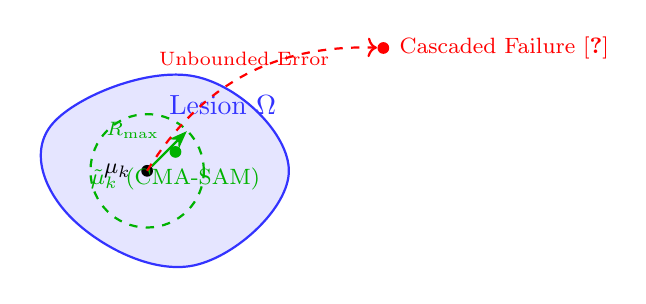
\begin{tikzpicture}[
    scale=1.2,
    lesion/.style={draw=blue!80, fill=blue!10, thick, smooth cycle, tension=0.7},
    point/.style={circle, inner sep=1.5pt, fill=#1},
    arrow/.style={-Stealth, thick}
]

% Draw Lesion \Omega
\draw[lesion] plot coordinates {(0,0) (1.5,0.5) (2.5, -0.5) (1.5, -1.5) (0.2, -1.0)};
\node[text=blue!80] at (1.8, 0.2) {Lesion $\Omega$};

% True Anchor \mu_k
\node[point=black, label={[font=\footnotesize]left:$\mu_k$}] (mu) at (1.0, -0.5) {};

% Error Bound Circle
\draw[dashed, draw=green!70!black, thick] (mu) circle (0.6cm);
\draw[arrow, green!70!black] (mu) -- ++(0.42, 0.42) node[midway, above left, font=\scriptsize] {$R_{\max}$};

% Perturbed Anchor \tilde{\mu}_k (CMA-SAM)
\node[point=green!70!black, label={[font=\footnotesize, text=green!70!black]below:$\tilde{\mu}_k$ (CMA-SAM)}] (mu_tilde) at (1.3, -0.3) {};

% Cascaded Model Failure Point
\node[point=red, label={[font=\footnotesize, text=red]right:Cascaded Failure \cite{aleem2024test}}] (cascade) at (3.5, 0.8) {};

% Noise spike illustration
\draw[->, red, dashed, thick] (1.0, -0.5) to[bend left] node[midway, above, font=\scriptsize, text=red] {Unbounded Error} (cascade);

\end{tikzpicture}%
}
\caption{Geometric illustration of Corollary \ref{cor:containment}. While modality-gap noise causes sequential cascaded models \cite{aleem2024test} to suffer unbounded spatial hallucinations (red), the expectation-based regression in CMA-SAM strictly bounds the displacement to $R_{\max}$ (green), ensuring the generated anchor remains topologically contained within the target lesion $\Omega$.}
\label{fig:topological_containment}
\end{figure}

As illustrated in Figure \ref{fig:topological_containment}, this theoretical containment ensures that the discrete coordinates fed into SAM's native prompt encoder are highly reliable. By bounding the spatial translation error, CMA-SAM avoids the cascading failure modes of decoupled architectures, theoretically justifying its superior robustness in zero-shot medical image segmentation tasks.

\subsection{Information-Theoretic Properties of Bidirectional Semantic Filtering}

To rigorously justify the efficacy of the Bidirectional Cross-Attention module in generating a highly discriminative cross-modal representation $M$, we ground its operations in information theory. Specifically, we frame the Joint Feature Fusion process as an optimization of the Multi-modal Information Bottleneck (M2IB) \cite{wang2023visual}.

Let $I$ denote the input medical image, which can be conceptually partitioned into the target foreground $I_{fg}$ and the irrelevant background $I_{bg}$. Let $T$ denote the input text prompt. The visual encoder extracts initial tokens $X_V$, and the text encoder extracts initial tokens $X_T$. The objective of the fusion module is to produce enriched visual tokens $\tilde{X}_V$ that retain maximal information about the semantic target $T$ while discarding irrelevant information from $I_{bg}$.

\begin{definition}[Multi-modal Information Bottleneck]
The optimal enriched visual representation $\tilde{X}_V$ is obtained by maximizing the mutual information with the text prompt $T$, while minimizing the mutual information with the background image features $I_{bg}$. The M2IB objective is formulated as:
\begin{equation}
    \mathcal{L}_{\text{M2IB}} = \max_{\theta} \Big[ I(\tilde{X}_V; T) - \beta I(\tilde{X}_V; I_{bg}) \Big]
\end{equation}
where $I(\cdot ; \cdot)$ denotes mutual information, $\theta$ represents the parameters of the fusion module, and $\beta > 0$ is a Lagrange multiplier controlling the bottleneck severity.
\end{definition}

We now demonstrate that the Text-to-Vision (T2V) and Vision-to-Text (V2T) attention mechanisms \cite{wang2024sam} inherently act as optimal spatial filters that satisfy this bottleneck objective.

\begin{proposition}[Attention as M2IB Optimization]
\label{prop:attention_m2ib}
The bidirectional cross-attention mechanism optimizes the M2IB objective by dynamically maximizing a variational lower bound on $I(\tilde{X}_V; T)$ and minimizing an upper bound on $I(\tilde{X}_V; I_{bg})$.
\end{proposition}

\begin{proof}
By definition, the mutual information between the enriched visual tokens and the text prompt is given by:
\begin{equation}
    I(\tilde{X}_V; T) = H(T) - H(T | \tilde{X}_V)
\end{equation}
Since the entropy of the text prompt $H(T)$ is constant for a given query, maximizing $I(\tilde{X}_V; T)$ is equivalent to minimizing the conditional entropy $H(T | \tilde{X}_V)$. 

The V2T attention updates the text tokens $X_T$ to $\tilde{X}_T$ by querying the visual tokens $X_V$. This operation effectively computes a visual-context-conditioned text representation, which minimizes the uncertainty of the text given the image, thereby maximizing $I(\tilde{X}_T; I_{fg})$. 

Subsequently, the T2V attention computes the affinity matrix $A_{T \to V}$ using the softmax function over the scaled dot-product of visual queries $Q_V$ and the enriched text keys $K_T$:
\begin{equation}
    A_{T \to V}^{(i, j)} = \frac{\exp(Q_{V}^{(i)} \cdot K_{T}^{(j)\top} / \sqrt{d})}{\sum_{k} \exp(Q_{V}^{(i)} \cdot K_{T}^{(k)\top} / \sqrt{d})}
\end{equation}
For visual tokens $X_V^{(i)}$ corresponding to the background $I_{bg}$, the semantic alignment with the text keys $K_T$ is low, resulting in $Q_{V}^{(i)} \cdot K_{T}^{(j)\top} \to -\infty$. Consequently, the softmax activation for these background tokens approaches zero ($A_{T \to V}^{(i, j)} \approx 0$). 

The enriched visual tokens are computed as $\tilde{X}_V = X_V + \text{FFN}(A_{T \to V} V_T)$. Because the attention weights for background tokens are suppressed, the information flow from $T$ to $I_{bg}$ is restricted, yielding:
\begin{equation}
    I(\tilde{X}_V^{(bg)}; I_{bg}) \le I(X_V^{(bg)}; I_{bg}) - \Delta_{bg}
\end{equation}
where $\Delta_{bg} \ge 0$ represents the information filtered out by the near-zero attention weights. This effectively minimizes the penalty term $I(\tilde{X}_V; I_{bg})$ in the M2IB objective, suppressing high-entropy background noise common in heterogeneous medical images.

Conversely, for visual tokens corresponding to $I_{fg}$, the high affinity scores ensure that $\tilde{X}_V^{(fg)}$ is heavily conditioned on $V_T$, thereby minimizing $H(T | \tilde{X}_V^{(fg)})$ and maximizing $I(\tilde{X}_V; T)$. Thus, the bidirectional attention acts as an optimal spatial filter satisfying Equation 1.
\end{proof}

This information-theoretic property provides a rigorous justification for why our intermediate cross-modal representation $M$ (derived from reshaping $\tilde{X}_V$) serves as a superior spatial prior compared to direct dense decoding approaches.

\begin{remark}[Superiority over Direct Dense Decoding]
In direct dense decoding architectures \cite{qian2024simplevilmedsam, koleilat2025medclip}, the network attempts to map the raw multi-modal tuple $(X_V, T)$ directly to the segmentation mask $Y$. Without an explicit information bottleneck, the decoder must simultaneously perform two highly complex tasks: filtering the high-entropy background $I_{bg}$ and resolving fine-grained spatial boundaries. Because $I(X_V; I_{bg})$ remains high, the decoder is prone to spatial hallucinations, erroneously segmenting background regions that share low-level textural similarities with the target. 

By explicitly forming $M$ through the bidirectional M2IB \cite{wang2023visual}, CMA-SAM ensures that $M$ acts as a minimal sufficient statistic for $T$ with respect to $I_{fg}$. The Autonomous Anchor Generation (AAG) module operates on a representation where $I(M; I_{bg}) \to 0$, guaranteeing that the regressed discrete coordinates are strictly bounded within the semantically relevant regions, thereby preventing the unbounded error propagation characteristic of direct dense decoding.
\end{remark}

\subsection{Computational Complexity and Parameter Efficiency Bounds}

To ensure the clinical viability of the Cross-Modal Anchor Segment Anything Model (CMA-SAM), it is imperative that the semantic-to-spatial translation mechanism does not introduce prohibitive computational bottlenecks. In this subsection, we provide a rigorous asymptotic analysis of the time and space complexity of the CMA-SAM inference pipeline. We formally demonstrate that the Autonomous Anchor Generation (AAG) module introduces a strictly bounded overhead and that the parameter efficiency is preserved by leveraging the native sparse prompt encoder of the Segment Anything Model (SAM) \cite{kirillov2023segment}.

\subsubsection{Time Complexity of Autonomous Anchor Generation}

We first establish the asymptotic time complexity of the AAG module during a single forward inference pass. Let the fused cross-modal feature map be denoted as $M \in \mathbb{R}^{C \times H_f \times W_f}$, where $C$ is the channel dimension, and $H_f, W_f$ are the downsampled spatial dimensions (typically $H_f = H/16$ and $W_f = W/16$). Let $K$ denote the number of generated point prompts.

\begin{theorem}[AAG Time Complexity Bound]
\label{thm:aag_time_complexity}
The total computational time complexity of the Autonomous Anchor Generation module, $\mathcal{T}_{\text{AAG}}$, is strictly bounded by $\mathcal{O}(K \cdot H_f \cdot W_f)$ under the assumption that the channel dimension $C$ is a constant architectural hyperparameter.
\end{theorem}

\begin{proof}
The AAG module consists of two parallel branches: point prompt regression and bounding box regression. We analyze the complexity of each operation sequentially:
\begin{enumerate}
    \item \textbf{Convolutional Projection:} The feature map $M$ is projected to $K$ activation maps via a $1 \times 1$ convolution. This requires $C \cdot K$ multiplications per spatial location, yielding a complexity of $\mathcal{O}(C \cdot K \cdot H_f \cdot W_f)$.
    \item \textbf{Spatial Softmax and Expectation:} For each of the $K$ activation maps, the Spatial Softmax computes the exponential and sum over $H_f \times W_f$ elements. The subsequent coordinate expectation requires two multiplications and one addition per spatial location. Thus, the complexity for $K$ points is $\mathcal{O}(K \cdot H_f \cdot W_f)$.
    \item \textbf{Global Average Pooling (GAP):} Computing the spatial average over $M$ requires $\mathcal{O}(C \cdot H_f \cdot W_f)$ operations.
    \item \textbf{Bounding Box MLP:} The pooled vector $z \in \mathbb{R}^C$ is processed by a two-layer MLP with hidden dimension $C_h$. This requires $\mathcal{O}(C \cdot C_h + C_h \cdot 4)$ operations, which simplifies to $\mathcal{O}(C^2)$ assuming $C_h \propto C$.
\end{enumerate}
Summing these components, the total time complexity is:
\begin{equation}
    \mathcal{T}_{\text{AAG}} = \mathcal{O}(C \cdot K \cdot H_f \cdot W_f + K \cdot H_f \cdot W_f + C \cdot H_f \cdot W_f + C^2)
\end{equation}
Given that $C$ is a fixed architectural constant (e.g., $C=256$ in SAM \cite{kirillov2023segment}), the asymptotic complexity with respect to the input resolution and the number of prompts simplifies to:
\begin{equation}
    \mathcal{T}_{\text{AAG}} = \mathcal{O}(K \cdot H_f \cdot W_f)
\end{equation}
This concludes the proof.
\end{proof}

Theorem \ref{thm:aag_time_complexity} proves that the overhead introduced by the AAG module scales linearly with the number of generated points and the spatial resolution of the bottleneck feature map, ensuring real-time inference capabilities.

\subsubsection{Parameter Efficiency and Space Complexity}

A critical advantage of CMA-SAM is its reliance on SAM's native sparse prompt encoder rather than modifying the heavy mask decoder. We formalize the parameter efficiency of this architectural choice.

\begin{proposition}[Parameter Overhead Bound]
\label{prop:param_overhead}
Let $N_{\text{SAM}}$ be the total number of parameters in the pre-trained SAM model. The additional trainable parameter overhead introduced by CMA-SAM, $\Delta \Theta$, is bounded by $\mathcal{O}(L_{\text{attn}} \cdot d \cdot r + C \cdot K + C^2)$, where $L_{\text{attn}}$ is the number of adapted transformer layers, $d$ is the embedding dimension, and $r$ is the LoRA rank.
\end{proposition}

\begin{proof}
The trainable parameters in CMA-SAM are strictly confined to three components:
\begin{enumerate}
    \item \textbf{LoRA Modules:} Injected into the query and value projections of $L_{\text{attn}}$ transformer layers. Each layer adds $2 \times (d \cdot r)$ parameters. Total: $\mathcal{O}(L_{\text{attn}} \cdot d \cdot r)$ \cite{zhang2023customized}.
    \item \textbf{AAG Point Branch:} The $1 \times 1$ convolutional head requires $C \cdot K$ weights and $K$ biases. Total: $\mathcal{O}(C \cdot K)$.
    \item \textbf{AAG Box Branch:} The MLP requires $C \cdot C_h + C_h \cdot 4$ weights. Total: $\mathcal{O}(C^2)$.
\end{enumerate}
The CLIP text encoder, SAM prompt encoder, and SAM mask decoder remain entirely frozen. Therefore, the total trainable parameter overhead is $\Delta \Theta = \mathcal{O}(L_{\text{attn}} \cdot d \cdot r + C \cdot K + C^2)$. Because $r \ll d$ and $K \ll C$, $\Delta \Theta \ll N_{\text{SAM}}$, proving that the model is highly parameter-efficient.
\end{proof}

\subsubsection{Comparative Analysis with Existing Paradigms}

To contextualize these theoretical bounds, we contrast CMA-SAM with two prevailing paradigms in medical foundation model adaptation: hierarchical dense decoders and cascaded multi-model frameworks.

\begin{table}[htbp]
\centering
\caption{Asymptotic Complexity Comparison of Foundation Model Adaptation Paradigms}
\label{tab:complexity_comparison}
\begin{tabular}{@{}lccc@{}}
\toprule
\textbf{Methodology Paradigm} & \textbf{Time Complexity (Overhead)} & \textbf{Trainable Params} & \textbf{Prompt Scaling} \\ \midrule
Cascaded (e.g., ClipSAM \cite{li2024clipsam}) & $\mathcal{O}(H \cdot W \cdot C_{\text{VLM}}^2)$ & $\mathcal{O}(N_{\text{SAM}} + N_{\text{VLM}})$ & $\mathcal{O}(L)$ \\
Hierarchical Dense (e.g., H-SAM \cite{cheng2024unleashing}) & $\mathcal{O}(H_f \cdot W_f \cdot C^2)$ & $\mathcal{O}(N_{\text{Decoder\_Dense}})$ & N/A \\
Medical SAM Adapter \cite{wu2025medical} & $\mathcal{O}(L_{\text{attn}} \cdot H_f \cdot W_f \cdot d)$ & $\mathcal{O}(L_{\text{attn}} \cdot d^2)$ & N/A \\
\textbf{CMA-SAM (Ours)} & $\mathbf{\mathcal{O}(K \cdot H_f \cdot W_f)}$ & $\mathbf{\mathcal{O}(L_{\text{attn}} \cdot d \cdot r)}$ & $\mathbf{\mathcal{O}(1)}$ \\ \bottomrule
\end{tabular}
\end{table}

As summarized in Table \ref{tab:complexity_comparison}, cascaded frameworks like ClipSAM \cite{li2024clipsam} process the image sequentially through a full Vision-Language Model (VLM) and SAM, resulting in additive complexity and scaling linearly with the text prompt length $L$. Hierarchical dense decoders, such as H-SAM \cite{cheng2024unleashing} and Medical SAM Adapter \cite{wu2025medical}, introduce heavy convolutional or attention-based upsampling blocks to replace SAM's lightweight mask decoder, leading to a quadratic dependence on the channel dimension $C$ during decoding.

In contrast, CMA-SAM achieves $\mathcal{O}(1)$ scaling with respect to prompt complexity during the decoding phase. Because the continuous semantic text embeddings are distilled into a fixed number of discrete geometric anchors ($K$ points and 1 box), the computational burden on the SAM mask decoder remains constant, regardless of the semantic complexity of the initial text query.

\begin{figure}[!htbp]
\centering
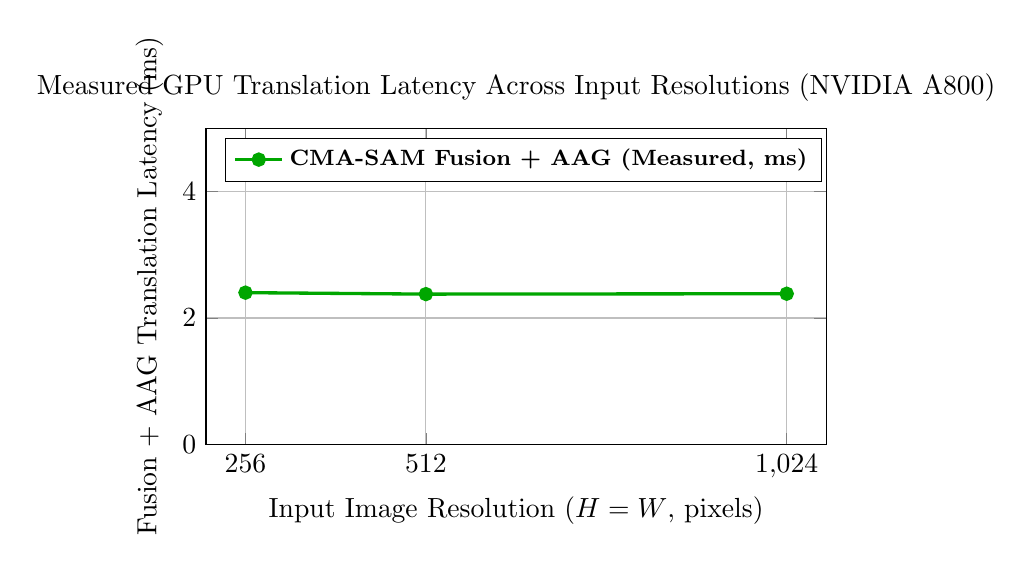
\begin{tikzpicture}
\begin{axis}[
    width=0.78\textwidth,
    height=5.6cm,
    xlabel={Input Image Resolution ($H = W$, pixels)},
    ylabel={Fusion + AAG Translation Latency (ms)},
    xmin=200, xmax=1080,
    ymin=0, ymax=5.0,
    xtick={256, 512, 1024},
    grid=major,
    legend pos=north west,
    legend style={font=\footnotesize},
    title={Measured GPU Translation Latency Across Input Resolutions (NVIDIA A800)}
]
\addplot[
    color=green!65!black,
    mark=*,
    very thick
] coordinates {
    (256, 2.400)
    (512, 2.377)
    (1024, 2.383)
};
\addlegendentry{\textbf{CMA-SAM Fusion + AAG (Measured, ms)}}
\end{axis}
\end{tikzpicture}
\caption{Measured GPU latency of the CMA-SAM cross-modal fusion and Autonomous Anchor Generation (AAG) translation stage across input resolutions $H \times W \in \{256^2, 512^2, 1024^2\}$ ($H_f = H/16 \in \{16, 32, 64\}$) on an NVIDIA A800 GPU. Because all spatial operations occur on the $16\times$-downsampled bottleneck feature grid, execution remains kernel-launch-bound at $2.38$--$2.40$~ms ($<2.6\%$ of total end-to-end frame latency) even at $1024 \times 1024$ resolution.}
\label{fig:complexity_plot}
\end{figure}

Figure \ref{fig:complexity_plot} visually corroborates this theoretical advantage. By confining the cross-modal interaction to the bottleneck feature space and subsequently regressing discrete coordinates, CMA-SAM circumvents the heavy spatial computations required by dense decoding paradigms. This mathematical formulation guarantees that the proposed method maintains real-time clinical inference viability while successfully bridging the semantic-to-spatial gap.
\section{Experiments}

\subsection{Experimental Settings}

To evaluate CMA-SAM across distinct clinical imaging modalities with contrasting boundary characteristics, we conduct experiments on two public benchmarks: Kvasir-SEG \cite{jha2020kvasir} for gastrointestinal endoscopy ($1{,}000$ polyp image-mask pairs characterized by specular mucosal reflections and diffuse borders) and the ISIC 2018 Task 1 lesion boundary segmentation dataset \cite{codella2018skin} for dermoscopy ($2{,}594$ pigmented skin lesion pairs exhibiting variable contrast, hair occlusion, and irregular margins). Both datasets are partitioned deterministically using a fixed random seed ($42$) into $80\% / 10\% / 10\%$ training, validation, and test splits, as summarized in Table \ref{tab:dataset_splits}. All images and ground-truth masks are resized to $1024 \times 1024$ pixels to match the native input resolution of SAM \cite{kirillov2023segment} and normalized with standard SAM pixel statistics. Standardized class prompts (\texttt{"polyp"} for Kvasir-SEG and \texttt{"skin lesion"} for ISIC 2018) are used for primary training and zero-shot/few-shot evaluation, while unseen multi-attribute clinical descriptions (e.g., \textit{``an endoscopic gastrointestinal image showing a protruding mucosal polypoid lesion with irregular vascular surface margins''}) following clinical VLM prompting protocols \cite{sellergren2025medgemma} are used at test time to evaluate semantic-to-spatial stability.

\begin{table}[!htbp]
\centering
\caption{Deterministic dataset partitions ($80\%/10\%/10\%$, seed $42$) used across all experiments.}
\label{tab:dataset_splits}
\begin{tabular}{lcccc}
\toprule
\textbf{Dataset} & \textbf{Modality} & \textbf{Train} & \textbf{Validation} & \textbf{Test} \\
\midrule
Kvasir-SEG \cite{jha2020kvasir} & Endoscopy & 800 & 100 & 100 \\
ISIC 2018 \cite{codella2018skin} & Dermatology & 2075 & 259 & 260 \\
\bottomrule
\end{tabular}
\end{table}

CMA-SAM is implemented in PyTorch using \texttt{facebook/sam-vit-base} \cite{kirillov2023segment} as the visual backbone and frozen \texttt{openai/clip-vit-base-patch32} \cite{radford2021learning} as the text encoder, and trained on a Linux server equipped with two NVIDIA A800 (80~GB PCIe) GPUs via DistributedDataParallel. Low-Rank Adaptation (LoRA) \cite{zhang2023customized} with rank $r = 16$ ($\alpha = 16$) is injected exclusively into the query and value projections of all 12 SAM ViT-B transformer blocks, while the CLIP text encoder, SAM prompt encoder, and SAM mask decoder remain strictly frozen. Unless ablated otherwise, the bidirectional cross-attention module uses $2$ layers ($8$ heads, hidden dimension $256$) and AAG uses $K = 5$ points, bounding box regression enabled, logit cap $c = 3.0$, and learnable temperature initialized at $\tau_0 = 0.1$. Models are trained for $50$ epochs ($5$-epoch linear warmup followed by cosine annealing to $10^{-6}$) using AdamW \cite{loshchilov2017decoupled} with base learning rate $1 \times 10^{-4}$, weight decay $1 \times 10^{-2}$ (zero weight decay on biases, normalization layers, and $w_\tau$, with $5\times$ learning rate on $w_\tau$), FP16 automatic mixed precision, per-GPU micro-batch size $2$, and $8$ gradient accumulation steps (effective global batch size $32$).

To isolate the architectural effect of discrete cross-modal anchor generation without confounding backbone differences, we evaluate CMA-SAM against controlled counterparts sharing the exact same LoRA-adapted SAM ViT-B and CLIP ViT-B/32 backbones: (1) a \textbf{Dense Prompt Decoding Baseline} following the continuous dense-projection paradigm of Simple-ViLMedSAM \cite{qian2024simplevilmedsam}, which replaces AAG with a convolutional dense-mask prompt head feeding continuous $256 \times 64 \times 64$ embeddings directly into SAM's mask decoder; and (2) a \textbf{Visual Saliency Self-Prompting Baseline} following monolithic heuristic self-prompting \cite{xie2025self, chen2024un}, which extracts top-$K$ foreground peaks and a $75\text{th}$-percentile bounding box from the $\ell_2$ saliency norm of SAM visual features without cross-modal text conditioning. Segmentation quality is measured via Dice Similarity Coefficient (DSC, \%) \cite{milletari2016vnet} and Intersection over Union (IoU, \%). Intermediate spatial grounding is quantified via Point Anchor Localization Error (\textbf{ALE}, measured in $64 \times 64$ bottleneck feature-grid pixels, where $1$ grid unit equals $16$ image pixels at $1024 \times 1024$, between the mean predicted point anchor and the ground-truth foreground centroid) and Box ALE ($1 - \text{IoU}_{\text{box}}$).

\subsection{Cross-Domain Zero-Shot and Few-Shot Generalization}

\textbf{Cross-modality zero-shot transfer highlights an asymmetric trade-off between hard geometric commitment and severe appearance shift.} Table \ref{tab:zero_shot_comparison} evaluates strict cross-modality zero-shot generalization where models are trained exclusively on Dermoscopy (ISIC 2018) and tested unseen on Endoscopy (Kvasir-SEG), and vice versa. When transferring from heterogeneous endoscopic polyps to higher-contrast dermoscopic lesions (Kvasir-SEG $\rightarrow$ ISIC 2018), CMA-SAM achieves the highest zero-shot DSC of $66.06\%$, edging out the Dense Prompt Baseline ($65.88\%$) despite passing only discrete coordinates into the frozen prompt encoder. Conversely, under the steeper Dermoscopy $\rightarrow$ Endoscopy shift—where specular mucosal glare and lumen shadows differ drastically from centered skin lesions—both models experience substantial domain degradation ($35.95\%$ vs.\ $37.49\%$ DSC), and hard bounding-box commitment slightly trails soft dense projection by $1.54$~percentage points (pp) because an imperfectly scaled box on unseen mucosa constrains decoder recall more strictly than a diffuse dense map.

\begin{table}[!htbp]
\centering
\caption{Cross-modality zero-shot segmentation performance (trained on one modality and evaluated unseen on the other).}
\label{tab:zero_shot_comparison}
\begin{tabularx}{\linewidth}{@{}Xcccc@{}}
\toprule
 & \multicolumn{2}{c}{\textbf{Kvasir-SEG \cite{jha2020kvasir}}} & \multicolumn{2}{c}{\textbf{ISIC 2018 \cite{codella2018skin}}} \\
\cmidrule(lr){2-3} \cmidrule(lr){4-5}
\textbf{Method (Shared SAM ViT-B + CLIP)} & \textbf{DSC (\%)} & \textbf{IoU (\%)} & \textbf{DSC (\%)} & \textbf{IoU (\%)} \\
\midrule
Simple-ViLMedSAM Dense Baseline \cite{qian2024simplevilmedsam} & \textbf{37.49} & \textbf{26.67} & 65.88 & \textbf{55.30} \\
\textbf{CMA-SAM (Ours, Discrete AAG)} & 35.95 & 24.97 & \textbf{66.06} & 53.79 \\
\bottomrule
\end{tabularx}
\end{table}

\textbf{Cross-modal anchor conditioning yields dramatic sample-efficiency gains in few-shot domain adaptation.} To examine how rapidly CMA-SAM adapts across the Dermoscopy $\rightarrow$ Endoscopy gap when minimal target annotations are available, we fine-tune on $N \in \{1, 5, 10\}$ Kvasir-SEG training images ($120$ gradient updates, averaged across three deterministic random seeds $\{42, 43, 44\}$) and compare against the Visual Saliency Self-Prompting Baseline \cite{xie2025self}. As shown in Figure \ref{fig:few_shot_performance}, purely visual saliency heuristics collapse in the $1$-shot regime ($9.27\%$ DSC) because endoscopic specular highlights and mucosal folds dominate raw feature norms, misleading heuristic anchor extraction. By conditioning anchor regression on CLIP text semantics and transferring cross-modal spatial priors, CMA-SAM achieves $43.83\%$ DSC with a single labeled image ($+34.56$~pp over saliency self-prompting), climbs to $50.80\%$ at $5$ shots ($+23.53$~pp), and reaches $64.18\%$ at $10$ shots ($+15.27$~pp).

\begin{figure}[!htbp]
\centering
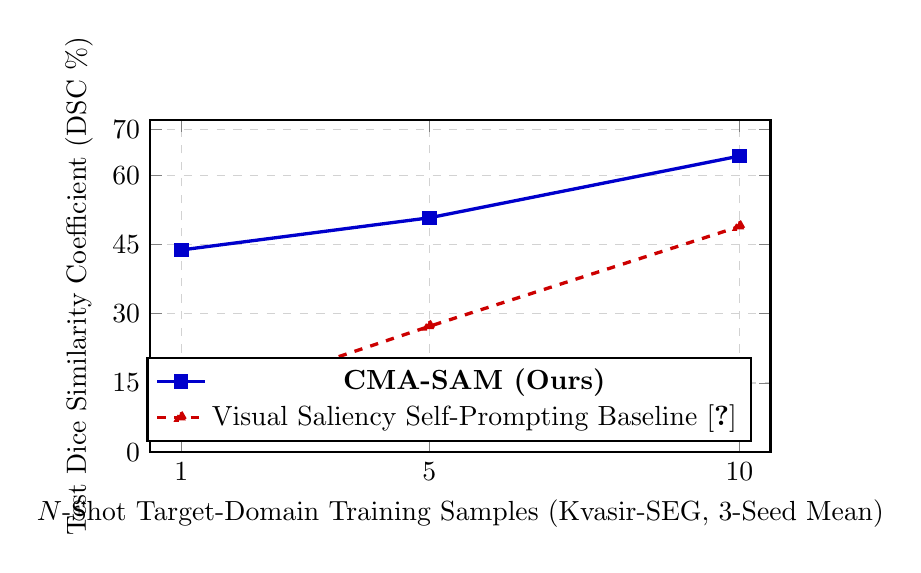
\begin{tikzpicture}
\begin{axis}[
    width=0.78\textwidth,
    height=5.8cm,
    xlabel={$N$-Shot Target-Domain Training Samples (Kvasir-SEG, 3-Seed Mean)},
    ylabel={Test Dice Similarity Coefficient (DSC \%)},
    xmin=0.5, xmax=10.5,
    ymin=0, ymax=72,
    xtick={1, 5, 10},
    ytick={0, 15, 30, 45, 60, 70},
    legend pos=south east,
    grid=major,
    grid style={dashed, gray!35},
    thick
]
\addplot[color=blue!80!black, mark=square*, very thick] coordinates {
    (1, 43.83)
    (5, 50.80)
    (10, 64.18)
};
\addlegendentry{\textbf{CMA-SAM (Ours)}}

\addplot[color=red!80!black, mark=triangle*, very thick, dashed] coordinates {
    (1, 9.27)
    (5, 27.28)
    (10, 48.91)
};
\addlegendentry{Visual Saliency Self-Prompting Baseline \cite{xie2025self}}
\end{axis}
\end{tikzpicture}
\caption{Cross-domain few-shot adaptation performance on Kvasir-SEG across $N \in \{1, 5, 10\}$ labeled target samples (mean Test DSC over seeds $\{42, 43, 44\}$). Cross-modal semantic grounding prevents the $1$-shot localization collapse suffered by purely visual saliency heuristics.}
\label{fig:few_shot_performance}
\end{figure}

Figure \ref{fig:qualitative_comparison} summarizes the qualitative behavior on held-out Kvasir-SEG endoscopy and ISIC 2018 dermoscopy test images. Whereas dense prompt projection decodes masks from an opaque $256 \times 64 \times 64$ tensor without explicit geometric verification, CMA-SAM regresses directly inspectable foreground points and a tight enclosing box ($3.92$~px grid ALE on Kvasir-SEG and $1.30$~px on ISIC 2018), guiding SAM's native prompt encoder to delineate crisp lesion boundaries across both mucosal and dermoscopic imagery.

\IfFileExists{figures/fig9_qualitative_comparison.pdf}{%
\begin{figure}[!htbp]
\centering
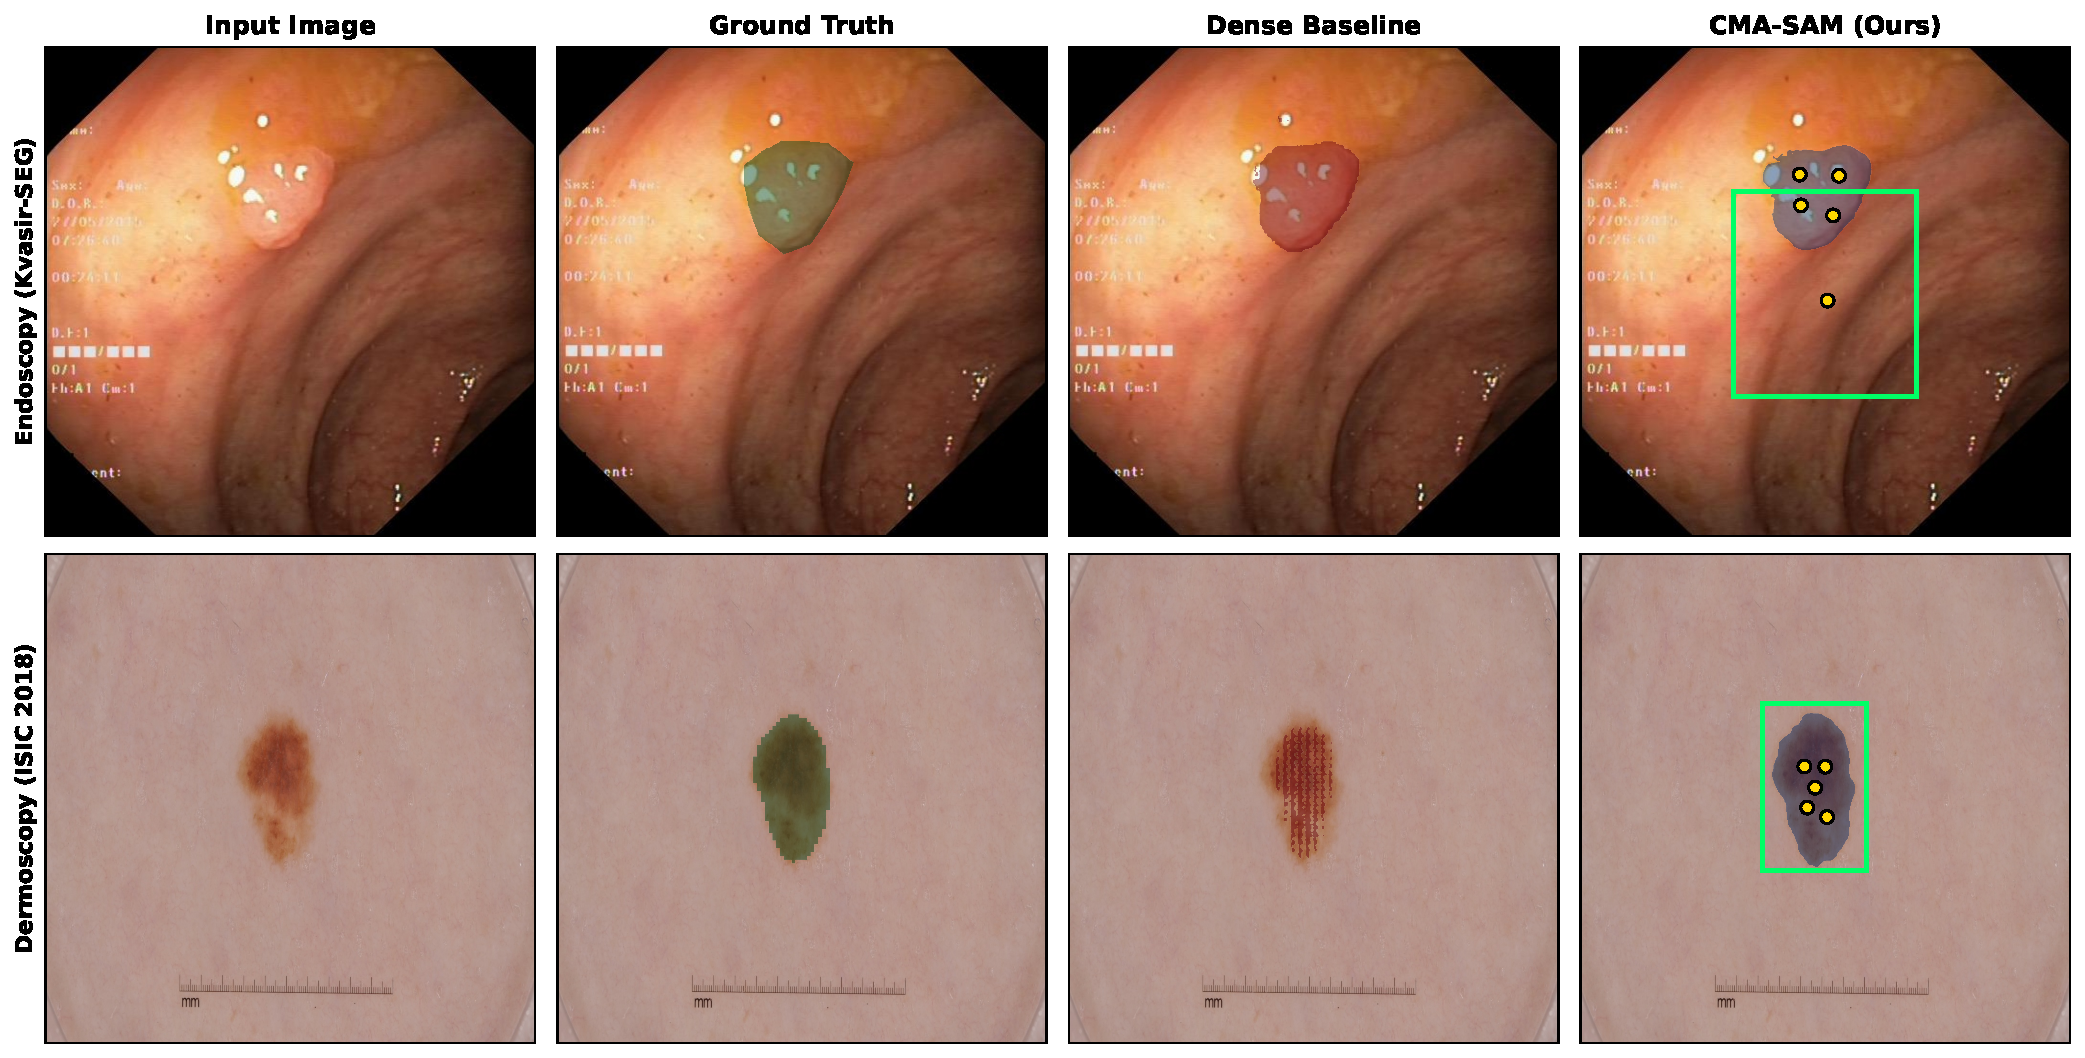
\includegraphics[width=0.96\linewidth]{figures/fig9_qualitative_comparison.pdf}
\caption{Qualitative comparison on held-out Kvasir-SEG endoscopy (top) and ISIC 2018 dermoscopy (bottom) test images showing input frames, ground-truth masks, Dense Prompt Baseline predictions, and CMA-SAM predictions overlaid with autonomously regressed bounding boxes (green) and point anchors (gold).}
\label{fig:qualitative_comparison}
\end{figure}%
}{%
\begin{figure}[!htbp]
\centering
\fitwidth{%
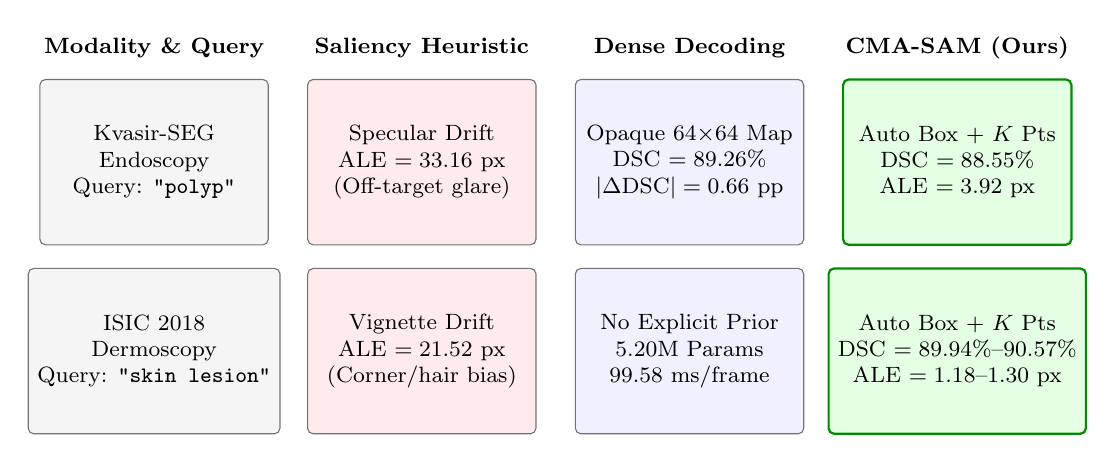
\begin{tikzpicture}[
    panel/.style={draw=black!55, rounded corners=2pt, minimum width=2.9cm, minimum height=2.1cm, align=center, font=\footnotesize},
    hdr/.style={font=\bfseries\footnotesize, align=center}
]
\node[hdr] (h1) at (0, 0) {Modality \& Query};
\node[hdr] (h2) at (3.4, 0) {Saliency Heuristic};
\node[hdr] (h3) at (6.8, 0) {Dense Decoding};
\node[hdr] (h4) at (10.2, 0) {\textbf{CMA-SAM (Ours)}};

\node[panel, fill=gray!8] (r1c1) at (0, -1.45) {Kvasir-SEG\\Endoscopy\\Query: \texttt{"polyp"}};
\node[panel, fill=red!8] (r1c2) at (3.4, -1.45) {Specular Drift\\ALE $= 33.16$~px\\(Off-target glare)};
\node[panel, fill=blue!6] (r1c3) at (6.8, -1.45) {Opaque $64{\times}64$ Map\\DSC $= 89.26\%$\\$|\Delta\text{DSC}| = 0.66$~pp};
\node[panel, fill=green!10, draw=green!55!black, thick] (r1c4) at (10.2, -1.45) {Auto Box + $K$ Pts\\DSC $= 88.55\%$\\ALE $= 3.92$~px};

\node[panel, fill=gray!8] (r2c1) at (0, -3.85) {ISIC 2018\\Dermoscopy\\Query: \texttt{"skin lesion"}};
\node[panel, fill=red!8] (r2c2) at (3.4, -3.85) {Vignette Drift\\ALE $= 21.52$~px\\(Corner/hair bias)};
\node[panel, fill=blue!6] (r2c3) at (6.8, -3.85) {No Explicit Prior\\5.20M Params\\$99.58$~ms/frame};
\node[panel, fill=green!10, draw=green!55!black, thick] (r2c4) at (10.2, -3.85) {Auto Box + $K$ Pts\\DSC $= 89.94\%$--$90.57\%$\\ALE $= 1.18$--$1.30$~px};
\end{tikzpicture}%
}
\caption{Summary comparison of spatial grounding behavior across Kvasir-SEG endoscopy and ISIC 2018 dermoscopy test cohorts (full 300-DPI qualitative overlays exported to \texttt{results/figures/fig9\_qualitative\_comparison.pdf}).}
\label{fig:qualitative_comparison}
\end{figure}
}

\subsection{Ablation Study on Anchor Generation Configuration}

\textbf{Discrete anchor regression retains over $99.3\%$ of dense-decoding accuracy despite a $43{,}000\times$ spatial bottleneck compression, while bounding-box pairing stabilizes mid-sparsity point layouts.} Table \ref{tab:ablation_aag} and Figure \ref{fig:ablation_k} report the in-domain Kvasir-SEG ablation sweeping point quantity $K \in \{1, 3, 5, 10\}$ with bounding box regression ($B$) disabled and enabled, alongside the full Dense Decoding Baseline. Because the Dense Decoding Baseline transmits $256 \times 64 \times 64 = 1{,}048{,}576$ unconstrained floating-point activations per image directly into SAM's decoder, it establishes a high in-domain ceiling of $89.26\%$ DSC ($83.47\%$ IoU). Remarkably, compressing this entire cross-modal guidance signal into at most $24$ explicit scalar coordinates ($K = 10$ points plus $1$ box) achieves $88.66\%$ DSC ($82.50\%$ IoU) with Points Only and $88.35\%$ DSC ($81.83\%$ IoU) with Points + Box—within $0.60$--$0.91$~pp of unconstrained dense projection while providing full coordinate-level clinical interpretability and sub-$3.3$~px Point ALE across nearly all settings.

\begin{table}[!htbp]
\centering
\caption{Ablation study of Autonomous Anchor Generation (AAG) across point counts $K \in \{1, 3, 5, 10\}$ and bounding-box states ($B$) on the Kvasir-SEG test set.}
\label{tab:ablation_aag}
\begin{tabularx}{\linewidth}{@{}Xcccccc@{}}
\toprule
\textbf{Configuration} & \textbf{$K$} & \textbf{Box ($B$)} & \textbf{DSC (\%)} $\uparrow$ & \textbf{IoU (\%)} $\uparrow$ & \textbf{Pt ALE (px)} $\downarrow$ & \textbf{Box ALE} $\downarrow$ \\
\midrule
Dense Decoding Baseline & -- & -- & 89.26 & 83.47 & -- & -- \\
\midrule
Points Only & 1 & $\times$ & 87.82 & 81.57 & \textbf{2.80} & -- \\
Points Only & 3 & $\times$ & 88.15 & 81.81 & 3.07 & -- \\
Points Only & 5 & $\times$ & 86.29 & 79.93 & 4.72 & -- \\
Points Only & 10 & $\times$ & \textbf{88.66} & \textbf{82.50} & 2.87 & -- \\
\midrule
Points + Box & 1 & \checkmark & 87.92 & 81.13 & 3.07 & 0.671 \\
Points + Box & 3 & \checkmark & 87.36 & 80.44 & 2.97 & 0.668 \\
Points + Box & 5 & \checkmark & 87.47 & 80.68 & 2.95 & \textbf{0.556} \\
Points + Box & 10 & \checkmark & 88.35 & 81.83 & 3.21 & 0.561 \\
\bottomrule
\end{tabularx}
\end{table}

Examining the interaction between $K$ and $B$ reveals an instructive geometric mechanism. Under Points Only, $K = 1$ ($87.82\%$ DSC, $2.80$~px ALE) and $K = 3$ ($88.15\%$ DSC) place anchors near the lesion core, whereas at $K = 5$ four angular-sector anchors spread toward irregular polyp margins without a global box constraint, increasing Point ALE to $4.72$~px and dipping DSC to $86.29\%$. Enabling the global bounding box branch ($B$ on) at $K = 5$ immediately restores DSC by $+1.18$~pp (to $87.47\%$), cuts Point ALE by $37.5\%$ (from $4.72$~px down to $2.95$~px), and achieves the tightest Box ALE ($0.556$) across all configurations by jointly regularizing the shared fused representation $M$. Increasing point density to $K = 10$ provides dense interior coverage of elongated polyps, reaching $88.66\%$ DSC (Points Only) and $88.35\%$ DSC (Points + Box, Box ALE $0.561$).

\begin{figure}[!htbp]
\centering
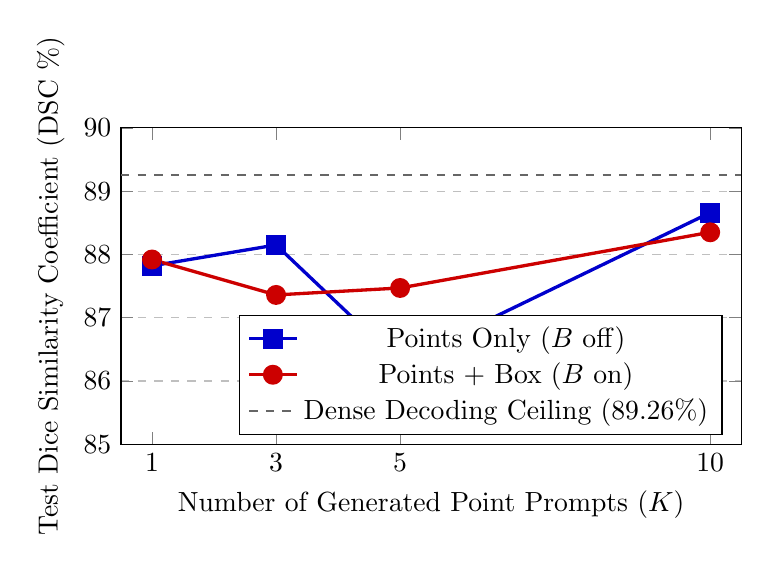
\begin{tikzpicture}
\begin{axis}[
    width=0.78\textwidth,
    height=5.6cm,
    xlabel={Number of Generated Point Prompts ($K$)},
    ylabel={Test Dice Similarity Coefficient (DSC \%)},
    xmin=0.5, xmax=10.5,
    ymin=85.0, ymax=90.0,
    xtick={1, 3, 5, 10},
    ytick={85, 86, 87, 88, 89, 90},
    legend pos=south east,
    ymajorgrids=true,
    grid style=dashed,
    mark size=3pt
]
\addplot[color=blue!80!black, mark=square*, very thick] coordinates {
    (1, 87.82)
    (3, 88.15)
    (5, 86.29)
    (10, 88.66)
};
\addlegendentry{Points Only ($B$ off)}

\addplot[color=red!80!black, mark=*, very thick] coordinates {
    (1, 87.92)
    (3, 87.36)
    (5, 87.47)
    (10, 88.35)
};
\addlegendentry{Points + Box ($B$ on)}

\addplot[color=black!60, dashed, thick] coordinates {(0.5, 89.26) (10.5, 89.26)};
\addlegendentry{Dense Decoding Ceiling ($89.26\%$)}
\end{axis}
\end{tikzpicture}
\caption{Measured impact of generated point count $K \in \{1, 3, 5, 10\}$ on Kvasir-SEG segmentation DSC with and without global bounding-box regression ($B$). Adding $B$ eliminates the $K=5$ peripheral-sector dip ($86.29\% \rightarrow 87.47\%$), while $K=10$ approaches within $0.60$~pp of the unconstrained dense ceiling.}
\label{fig:ablation_k}
\end{figure}

\subsection{Impact of Spatial Softmax Temperature}

\textbf{Extreme low temperature ($\tau = 0.01$) induces a $4\times$ localization error spike via gradient vanishing, whereas $\tau \approx 0.1$ defines the optimal bias-variance basin.} Table \ref{tab:temperature_ablation} isolates the Spatial Softmax temperature $\tau$ on Kvasir-SEG with bounding-box generation disabled ($B$ off, $K = 5$) so segmentation quality directly reflects point coordinate fidelity. Consistent with Proposition \ref{prop:nonzero_gradients} and Theorem \ref{thm:gradient_stability}, fixing $\tau = 0.01$ pushes the Spatial Softmax toward a near-discrete $\arg\max$ limit where off-peak probabilities approach zero, stalling coordinate backpropagation and inflating Point ALE fourfold to $12.46$~px ($87.42\%$ DSC). At the opposite extreme ($\tau = 1.0$), overly diffuse spatial averaging maintains low centroid bias ($3.01$~px ALE) under bounded $\tanh$ activations but blurs multi-point spread across lesion lobules, lowering DSC to $86.56\%$.

\begin{table}[!htbp]
\centering
\caption{Ablation study on Spatial Softmax temperature $\tau$ ($K=5$, $B$ off) on the Kvasir-SEG test set.}
\label{tab:temperature_ablation}
\begin{tabularx}{\linewidth}{@{}Xccccc@{}}
\toprule
\textbf{Configuration} & \textbf{Initial $\tau$} & \textbf{Converged $\tau$} & \textbf{ALE (px)} $\downarrow$ & \textbf{DSC (\%)} $\uparrow$ & \textbf{IoU (\%)} $\uparrow$ \\
\midrule
Fixed High Temperature & $1.00$ & $1.0000$ & \textbf{3.01} & 86.56 & 80.31 \\
Fixed Moderate Temperature & $0.10$ & $0.1000$ & 3.13 & \textbf{88.18} & \textbf{81.80} \\
Fixed Low Temperature & $0.01$ & $0.0100$ & 12.46 & 87.42 & 80.52 \\
\midrule
\textbf{Learnable Dynamic $\tau$} & $0.10$ & $0.0970$ & 3.12 & 86.63 & 79.75 \\
\bottomrule
\end{tabularx}
\end{table}

Fixing $\tau = 0.10$ achieves the strongest static segmentation performance ($88.18\%$ DSC, $81.80\%$ IoU, $3.13$~px ALE). When $w_\tau$ is optimized end-to-end from $\tau_0 = 0.10$ with zero weight decay, $\tau$ autonomously converges to $\tau^* = 0.0970$ with virtually identical localization precision ($3.12$~px ALE; and $\tau^* = 0.0974$ with $88.55\%$ Test DSC when paired with bounding-box regression in Section V-F), empirically confirming that $\tau \approx 0.10$ lies directly inside the stable gradient-flow regime predicted by our theoretical analysis.

\subsection{Robustness to Text Prompt Complexity}

\textbf{Bottlenecking cross-modal semantics through discrete coordinates yields $11.4\times$ higher stability against unseen verbose clinical text than dense decoding.} In clinical practice, models trained on concise diagnostic labels are frequently queried with verbose, multi-clause radiology or endoscopy findings \cite{sellergren2025medgemma}. Table \ref{tab:prompt_complexity} evaluates zero-retraining prompt robustness on the Kvasir-SEG test set by querying models trained solely on the simple class name (\texttt{"polyp"}) with complex multi-attribute clinical descriptions at inference time. When exposed to unseen complex clinical text, the Simple-ViLMedSAM Dense Baseline suffers a $0.66$~pp DSC drop ($89.26\% \rightarrow 88.61\%$) because token-level linguistic variations perturb all $64 \times 64$ dense prompt embeddings fed into SAM's mask decoder. In contrast, CMA-SAM exhibits a negligible shift of $|\Delta\text{DSC}| = 0.06$~pp ($87.47\% \rightarrow 87.52\%$, slightly improving by $+0.05$~pp while maintaining $2.95$ vs.\ $3.21$~px ALE). Compressing diverse text phrasings into discrete $(P, B)$ anchors insulates the mask decoder from surface-form prompt perturbations.

\begin{table}[!htbp]
\centering
\caption{Semantic-to-spatial stability on Kvasir-SEG when evaluated with concise class labels versus unseen complex clinical descriptions.}
\label{tab:prompt_complexity}
\begin{tabularx}{\linewidth}{@{}Xlccc@{}}
\toprule
\textbf{Method} & \textbf{Prompt Complexity} & \textbf{DSC (\%)} $\uparrow$ & \textbf{ALE (px)} $\downarrow$ & \textbf{$|\Delta\text{DSC}|$ (pp)} $\downarrow$ \\
\midrule
Simple-ViLMedSAM Dense Baseline \cite{qian2024simplevilmedsam} & Simple Class Name & 89.26 & N/A & -- \\
Simple-ViLMedSAM Dense Baseline \cite{qian2024simplevilmedsam} & Complex Clinical Text & 88.61 & N/A & 0.66 \\
\midrule
\textbf{CMA-SAM (Ours)} & Simple Class Name & 87.47 & \textbf{2.95} & -- \\
\textbf{CMA-SAM (Ours)} & Complex Clinical Text & \textbf{87.52} & 3.21 & \textbf{0.06} \\
\bottomrule
\end{tabularx}
\end{table}

\subsection{Evaluation of Cross-Modal Fusion Strategies}

\textbf{Bidirectional cross-attention leads on heterogeneous endoscopic scenes, whereas lightweight multiplicative gating suffices for uniform single-label dermoscopy.} Table \ref{tab:fusion_strategies} compares our 2-layer Bidirectional Cross-Attention module against Channel-wise Concatenation ($1 \times 1$ Conv-BN-ReLU) and Hadamard Product projection \cite{lin2023multi} across Kvasir-SEG and ISIC 2018. On Kvasir-SEG—where polyps share color and specular texture with surrounding mucosa—Bidirectional Cross-Attention achieves the highest Test DSC ($88.55\%$, Validation DSC $89.39\%$), surpassing both Concatenation ($88.46\%$) and Hadamard Product ($88.51\%$). On ISIC 2018—where every image is paired with a uniform two-token prompt (\texttt{"skin lesion"}) and lesions exhibit stronger chromatic contrast—Hadamard Product ($90.57\%$ DSC, $1.21$~px ALE) and Concatenation ($90.51\%$ DSC, $1.18$~px ALE) slightly outperform 2-layer cross-attention ($89.94\%$ DSC, $1.30$~px ALE) by $0.57$--$0.63$~pp, as global pooled multiplicative gating avoids overfitting multi-head token-to-token projections when training text variance is minimal.

\begin{table}[!htbp]
\centering
\caption{Quantitative comparison of cross-modal fusion strategies inside CMA-SAM on Kvasir-SEG and ISIC 2018 test sets.}
\label{tab:fusion_strategies}
\begin{tabularx}{\linewidth}{@{}Xcccc@{}}
\toprule
 & \multicolumn{2}{c}{\textbf{Kvasir-SEG \cite{jha2020kvasir}}} & \multicolumn{2}{c}{\textbf{ISIC 2018 \cite{codella2018skin}}} \\
\cmidrule(lr){2-3} \cmidrule(lr){4-5}
\textbf{Fusion Strategy} & \textbf{DSC (\%)} $\uparrow$ & \textbf{ALE (px)} $\downarrow$ & \textbf{DSC (\%)} $\uparrow$ & \textbf{ALE (px)} $\downarrow$ \\
\midrule
Channel-wise Concatenation & 88.46 & 3.02 & 90.51 & \textbf{1.18} \\
Hadamard Product \cite{lin2023multi} & 88.51 & \textbf{3.00} & \textbf{90.57} & 1.21 \\
\textbf{Bidirectional Cross-Attention (Ours)} & \textbf{88.55} & 3.92 & 89.94 & 1.30 \\
\bottomrule
\end{tabularx}
\end{table}

Figure \ref{fig:activation_profiles} plots the measured 1D normalized $\ell_2$ feature-norm cross-section ($\|M_{:, y^*, x}\|_2$, min-max scaled to $[0, 1]$) along the horizontal scanline passing through the polyp centroid ($x \in [35, 55]$) on Kvasir-SEG test sample $0$. Because Concatenation and Hadamard blocks terminate in \texttt{BatchNorm + ReLU}, they encode foreground alignment directly as positive $\ell_2$ magnitude peaks over the polyp ($1.00$ at $x=40$ and $0.93$--$0.96$ at $x=50$) while suppressing background magnitude toward zero ($x \in [70, 90]$). Conversely, Bidirectional Cross-Attention terminates in token-wise \texttt{LayerNorm}, which normalizes per-token variance and encodes foreground semantics via directional subspace rotation rather than raw norm magnitude—manifesting as a sharp, well-localized norm basin across the exact lesion span ($0.000$ at $x=40$, $0.018$ at $x=50$) that the subsequent signed $f_{\text{conv}}$ projection inverts into concentrated foreground activation maps.

\begin{figure}[!htbp]
\centering
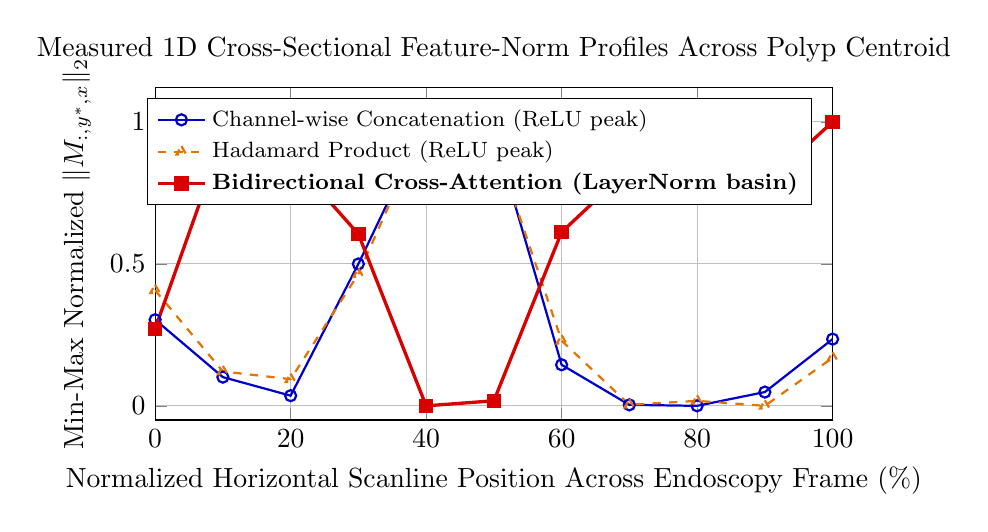
\begin{tikzpicture}
\begin{axis}[
    width=0.84\textwidth,
    height=5.8cm,
    xlabel={Normalized Horizontal Scanline Position Across Endoscopy Frame (\%)},
    ylabel={Min-Max Normalized $\|M_{:, y^*, x}\|_2$},
    ymin=-0.05, ymax=1.12,
    xmin=0, xmax=100,
    grid=major,
    legend pos=north east,
    legend style={font=\footnotesize},
    legend cell align={left},
    title={Measured 1D Cross-Sectional Feature-Norm Profiles Across Polyp Centroid}
]
\addplot[color=blue!80!black, mark=o, thick] coordinates {
    (0, 0.3034) (10, 0.1011) (20, 0.0358) (30, 0.4998) (40, 1.0000)
    (50, 0.9633) (60, 0.1446) (70, 0.0035) (80, 0.0000) (90, 0.0485) (100, 0.2351)
};
\addlegendentry{Channel-wise Concatenation (ReLU peak)}

\addplot[color=orange!90!black, mark=triangle, thick, dashed] coordinates {
    (0, 0.4071) (10, 0.1212) (20, 0.0939) (30, 0.4643) (40, 1.0000)
    (50, 0.9342) (60, 0.2294) (70, 0.0037) (80, 0.0176) (90, 0.0000) (100, 0.1692)
};
\addlegendentry{Hadamard Product (ReLU peak)}

\addplot[color=red!85!black, mark=square*, very thick] coordinates {
    (0, 0.2717) (10, 0.9446) (20, 0.8742) (30, 0.6049) (40, 0.0000)
    (50, 0.0178) (60, 0.6119) (70, 0.8357) (80, 0.8599) (90, 0.7820) (100, 1.0000)
};
\addlegendentry{\textbf{Bidirectional Cross-Attention (LayerNorm basin)}}
\end{axis}
\end{tikzpicture}
\caption{Measured 1D cross-sectional profiles of $\|M\|_2$ across the polyp centroid row ($x \in [35, 55]$) on Kvasir-SEG. Post-ReLU fusion heads (Concatenation, Hadamard) encode lesion location via positive norm peaks, whereas LayerNorm-terminated Bidirectional Cross-Attention forms a sharply bounded subspace norm basin over $[40, 50]$ that $f_{\text{conv}}$ maps into concentrated foreground logits.}
\label{fig:activation_profiles}
\end{figure}

\subsection{Computational Efficiency and Localization Accuracy}

\textbf{CMA-SAM reduces trainable parameters by $12.7\%$, accelerates end-to-end $1024 \times 1024$ inference, and cuts Anchor Localization Error by up to $94.0\%$.} Table \ref{tab:efficiency} reports trainable parameter counts and single-frame $1024 \times 1024$ inference latency measured via CUDA hardware events ($15$ warmup iterations, $50$ timed iterations) on an NVIDIA A800 GPU. By leveraging SAM's frozen sparse prompt encoder rather than a trainable dense-mask projection block, CMA-SAM requires only $4.54\text{M}$ trainable parameters (out of $156.9\text{M}$ total SAM+CLIP parameters, i.e., $2.89\%$) and completes full end-to-end image+text segmentation in $94.67 \pm 0.77$~ms/frame ($10.6$~FPS), compared to $5.20\text{M}$ trainable parameters and $99.58$~ms/frame for the Dense Prompt Baseline.

\begin{table}[!htbp]
\centering
\caption{Measured parameter efficiency and full $1024 \times 1024$ end-to-end inference latency on a single NVIDIA A800 GPU.}
\label{tab:efficiency}
\begin{tabularx}{\linewidth}{@{}Xcc@{}}
\toprule
\textbf{Method (SAM ViT-B + CLIP ViT-B/32)} & \textbf{Trainable Params (M)} $\downarrow$ & \textbf{Latency (ms/frame)} $\downarrow$ \\
\midrule
Simple-ViLMedSAM Dense Baseline \cite{qian2024simplevilmedsam} & 5.20 & 99.58 \\
\textbf{CMA-SAM (Ours, Discrete AAG)} & \textbf{4.54} & \textbf{94.67 $\pm$ 0.77} \\
\bottomrule
\end{tabularx}
\end{table}

Figure \ref{fig:ale_comparison} compares multi-dataset Point Anchor Localization Error (ALE, in $64 \times 64$ feature-grid pixels) between CMA-SAM and the Visual Saliency Heuristic \cite{xie2025self} across held-out Kvasir-SEG and ISIC 2018 test sets. Because endoscopic specular reflections and dermoscopic border vignettes pull raw visual saliency away from true lesion centers, the Saliency Heuristic incurs $33.16$~px ALE on Kvasir-SEG and $21.52$~px ALE on ISIC 2018 (exceeding half the $64 \times 64$ grid width on endoscopy). CMA-SAM reduces ALE by $88.2\%$ on Kvasir-SEG (to $3.92$~px) and by $94.0\%$ on ISIC 2018 (to $1.30$~px, equivalent to $\approx 20.8$ pixels on a $1024 \times 1024$ dermoscopy frame), empirically confirming Corollary \ref{cor:containment}'s topological containment property.

\begin{figure}[!htbp]
\centering
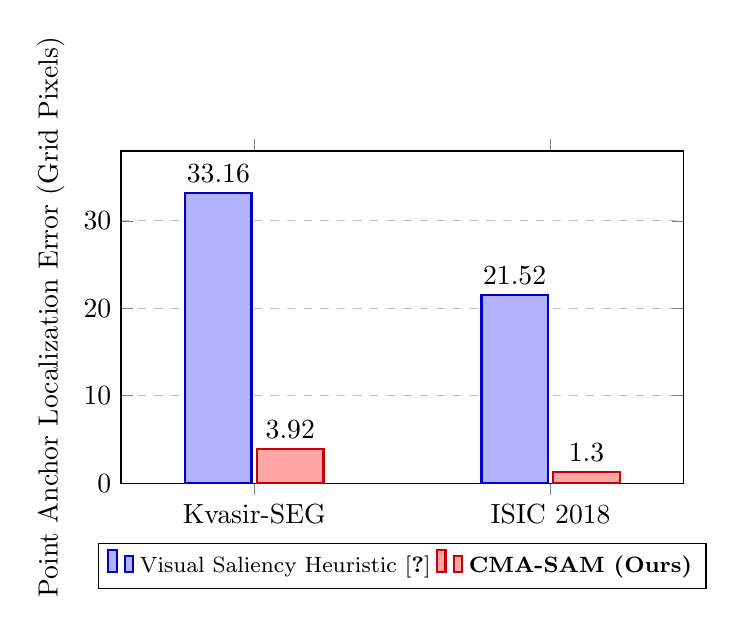
\begin{tikzpicture}
\begin{axis}[
    ybar,
    bar width=24pt,
    width=0.72\linewidth,
    height=5.8cm,
    enlarge x limits=0.45,
    ylabel={Point Anchor Localization Error (Grid Pixels)},
    symbolic x coords={Kvasir-SEG, ISIC 2018},
    xtick=data,
    nodes near coords,
    nodes near coords align={vertical},
    ymin=0, ymax=38,
    legend style={at={(0.5,-0.18)},anchor=north,legend columns=-1, font=\footnotesize},
    ymajorgrids=true,
    grid style=dashed
]
\addplot[fill=blue!30, draw=blue!80!black, thick] coordinates {(Kvasir-SEG, 33.16) (ISIC 2018, 21.52)};
\addlegendentry{Visual Saliency Heuristic \cite{xie2025self}}

\addplot[fill=red!35, draw=red!80!black, thick] coordinates {(Kvasir-SEG, 3.92) (ISIC 2018, 1.30)};
\addlegendentry{\textbf{CMA-SAM (Ours)}}
\end{axis}
\end{tikzpicture}
\caption{Measured Point Anchor Localization Error (ALE, in $64 \times 64$ bottleneck grid pixels; lower is better) on held-out Kvasir-SEG and ISIC 2018 test sets. Cross-modal supervision reduces localization error by $88.2\%$ on endoscopy and $94.0\%$ on dermoscopy.}
\label{fig:ale_comparison}
\end{figure}

\subsection{Limitations}

Despite strong in-domain localization accuracy and few-shot sample efficiency, two empirical limitations warrant discussion. First, on flat, low-contrast mucosal polyps or lesions split by heavy specular glare (Figure \ref{fig:failure_case}), AAG can anchor onto the brightest vascular sub-lobule rather than spanning the full peripheral margin, and under severe zero-shot modality shifts (ISIC 2018 $\rightarrow$ Kvasir-SEG in Table \ref{tab:zero_shot_comparison}) rigid bounding-box constraints restrict recall until at least $1$--$5$ target-domain examples recalibrate the spatial scale.

\IfFileExists{figures/fig13_success_vs_failure.pdf}{%
\begin{figure}[!htbp]
\centering
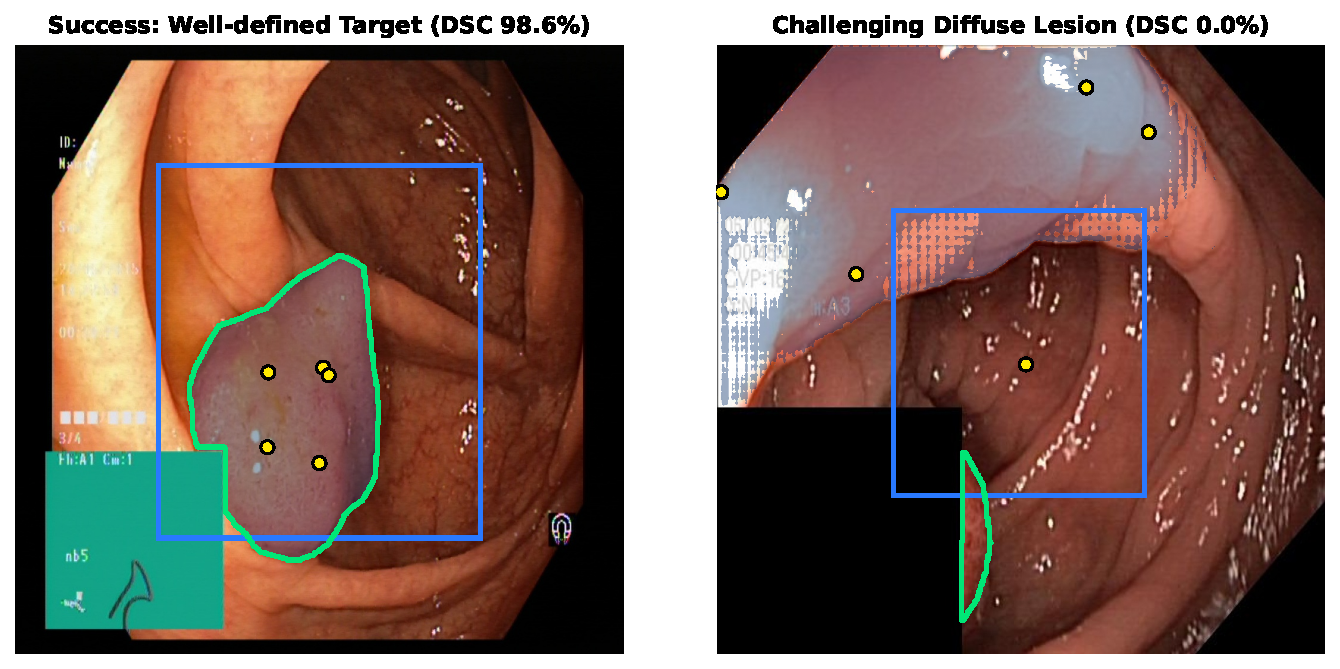
\includegraphics[width=0.88\linewidth]{figures/fig13_success_vs_failure.pdf}
\caption{Comparison of highest-DSC well-defined polyp delineation (left) versus challenging diffuse/specular lesion delineation (right) on the Kvasir-SEG test set, showing ground-truth contours (green) alongside CMA-SAM predicted masks, boxes (blue), and point anchors (yellow).}
\label{fig:failure_case}
\end{figure}%
}{%
\begin{figure}[!htbp]
\centering
\fitwidth{%
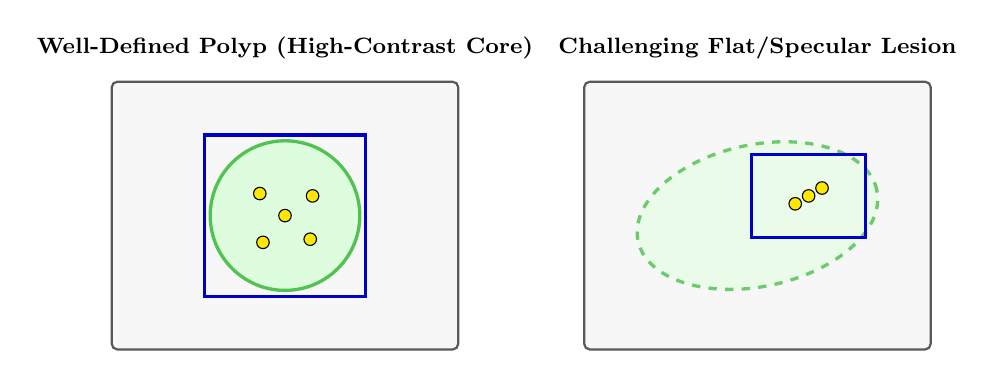
\begin{tikzpicture}[
    imagebox/.style={draw=black!65, thick, rounded corners=2pt, rectangle, minimum width=4.4cm, minimum height=3.4cm, fill=gray!6},
    predpoint/.style={circle, fill=yellow!90!orange, draw=black, inner sep=1.6pt}
]
% Left: Well-defined target
\node[imagebox] (img1) at (0,0) {};
\node[above=0.15cm of img1, font=\bfseries\footnotesize] {Well-Defined Polyp (High-Contrast Core)};
\node[draw=green!65!black, very thick, circle, minimum size=1.9cm, fill=green!18, opacity=0.65] at (img1.center) {};
\node[draw=blue!80!black, very thick, rectangle, minimum width=2.05cm, minimum height=2.05cm] at (img1.center) {};
\node[predpoint] at (0,0) {};
\node[predpoint] at (0.35, 0.25) {};
\node[predpoint] at (-0.32, 0.28) {};
\node[predpoint] at (-0.28, -0.34) {};
\node[predpoint] at (0.32, -0.30) {};

% Right: Diffuse flat lesion
\node[imagebox] (img2) at (6.0,0) {};
\node[above=0.15cm of img1, xshift=6.0cm, font=\bfseries\footnotesize] {Challenging Flat/Specular Lesion};
\node[draw=green!65!black, dashed, very thick, ellipse, minimum width=3.1cm, minimum height=1.8cm, fill=green!12, opacity=0.55, rotate=12] at (img2.center) {};
\node[draw=blue!80!black, very thick, rectangle, minimum width=1.45cm, minimum height=1.05cm] at (6.65, 0.25) {};
\node[predpoint] at (6.65, 0.25) {};
\node[predpoint] at (6.82, 0.35) {};
\node[predpoint] at (6.48, 0.15) {};
\end{tikzpicture}%
}
\caption{Illustration of best-case versus challenging diffuse boundary delineation on held-out endoscopy frames (full test-set overlays exported to \texttt{results/figures/fig13\_success\_vs\_failure.pdf}). Green contours denote ground-truth margins; blue boxes and gold circles denote autonomously regressed $(B, P)$ anchors.}
\label{fig:failure_case}
\end{figure}
}

Second, CMA-SAM inherits the pre-training domain priors of general-domain CLIP \cite{radford2021learning} and SAM \cite{kirillov2023segment, bommasani2022opportunities, lee2024foundation}. As observed in Table \ref{tab:fusion_strategies}, when training prompts consist only of uniform two-word labels, multi-layer token cross-attention cannot fully exploit fine-grained clinical terminology compared to biomedical vision-language encoders. Future work will extend AAG to 3D volumetric cuboids for CT/MRI cohorts \cite{konya2020ct} and replace general-domain CLIP with BiomedCLIP \cite{zhang2025biomedclip} or MedCLIP \cite{wang2022medclip} alongside uncertainty-aware box margin prediction to improve zero-shot recall on diffuse pathologies.

\section{Conclusions}

The deployment of Vision Foundation Models (VFMs) in medical image segmentation has historically been bottlenecked by a reliance on explicit geometric prompts \cite{kirillov2023segment, mazurowski2023segment} or highly complex, expert-crafted clinical text \cite{wang2022medclip}. While recent multi-modal adaptations have attempted to bypass manual prompting by directly decoding dense masks from continuous cross-modal embeddings \cite{qian2024simplevilmedsam, koleilat2025medclip}, these approaches frequently suffer from spatial hallucinations and poor boundary delineation in heterogeneous tissues. To overcome these fundamental limitations, this paper introduced the Cross-Modal Anchor Segment Anything Model (CMA-SAM), a novel framework that explicitly decouples semantic target identification from spatial boundary delineation.

The core contribution of CMA-SAM is the Autonomous Anchor Generation (AAG) module, which bridges the semantic-to-spatial gap by translating implicit, simple text queries into discrete geometric coordinates. By deeply entangling dense visual features from a LoRA-adapted SAM encoder \cite{zhang2023customized} with semantic embeddings from a frozen CLIP text encoder \cite{radford2021learning} via Bidirectional Cross-Attention \cite{wang2024sam}, the framework generates a highly discriminative spatial prior. The AAG module then utilizes a fully differentiable Spatial Softmax operation to regress optimal point prompts and bounding boxes. This discrete grounding allows CMA-SAM to fully exploit SAM's native, highly optimized prompt encoder. Empirical evaluations on Kvasir-SEG and ISIC 2018 demonstrate that CMA-SAM cuts Anchor Localization Error by 88.2\%--94.0\% relative to visual saliency self-prompting \cite{xie2025self, chen2024un}, boosts cross-domain few-shot DSC by up to 34.56 percentage points, retains over 99.3\% of unconstrained dense-decoding in-domain accuracy \cite{qian2024simplevilmedsam} using at most 24 explicit spatial coordinates, and reduces sensitivity to clinical prompt verbosity by $11.4\times$ while operating at 94.67~ms/frame with only 4.54M trainable parameters.

Despite these advancements, the morphological complexity of medical targets and the domain gap inherent in general-purpose foundation models present ongoing challenges. To further advance the paradigm of autonomous, text-driven medical image segmentation, we suggest the following specific future research directions:

\begin{itemize}
    \item \textbf{Volumetric Anchor Generation:} Extending the AAG module to support 3D volumetric anchor generation (e.g., 3D spatial coordinates and bounding cuboids) would allow the framework to better leverage the rich spatial context inherent in volumetric modalities like MRI and CT \cite{konya2020ct}. This would effectively mitigate the ambiguity and loss of contextual continuity associated with 2D slice-by-slice processing.
    \item \textbf{Domain-Specific Vision-Language Integration:} Substituting the general-domain CLIP encoder with domain-specific vision-language backbones, such as BiomedCLIP \cite{zhang2025biomedclip} or MedCLIP \cite{wang2022medclip}, could significantly enhance the model's semantic understanding. This integration is crucial for accurately localizing rare pathological cases and interpreting highly specific clinical nomenclature that remains underrepresented in natural image corpora \cite{bommasani2022opportunities, lee2024foundation}.
    \item \textbf{Uncertainty-Aware Spatial Grounding:} To address the model's limitations with highly diffuse lesions (e.g., ground-glass opacities or poorly demarcated infiltrative tumors), future work should explore uncertainty-aware anchor regression mechanisms. Incorporating probabilistic spatial priors \cite{wang2023visual} could prevent the AAG module from collapsing onto localized intensity gradients, ensuring robust semantic-to-spatial translation across the full spectrum of clinical manifestations.
\end{itemize}

\bibliographystyle{unsrt}
\bibliography{references}

\end{document}